%%
%% ****** Generated 18.03.21 by LJM TeX-constructor******
%%Sat 25 september
\documentclass[
11pt,%
tightenlines,%
twoside,%
onecolumn,%
nofloats,%
nobibnotes,%
nofootinbib,%
superscriptaddress,%
noshowpacs,%
centertags]%
{revtex4}
\usepackage{ljm}
%\setcounter{page}{3}
%\usepackage{subfig}
\usepackage{amssymb}
\usepackage{bm}
\usepackage{amsmath}
\usepackage{autonum}
\usepackage{url}
\DeclareMathOperator*{\argmax}{arg\,max}
\DeclareMathOperator*{\argmin}{arg\,min}
\newcommand*{\No}{No.}

\begin{document}
\titlerunning{Sample size estimation} % for running heads
%Grabovoy, Gadaev, Motrenko, Strijov
\title{Numerical methods of sufficient sample size estimation for generalised linear models}
\author{\firstname{A.\,V.}~\surname{Grabovoy}}
\email[E-mail: ]{grabovoy.av@phystech.edu}
\affiliation{Moscow Institute of Physics and Technology, 9 Institutskiy per., Dolgoprudny, Moscow Region, 141701, Russian Federation}
\author{\firstname{T.\,T.}~\surname{Gadaev}}
\email[E-mail: ]{gadaev.tt@phystech.edu}
\affiliation{Moscow Institute of Physics and Technology, 9 Institutskiy per., Dolgoprudny, Moscow Region, 141701, Russian Federation}
\author{\firstname{A.\,P.}~\surname{Motrenko}}
\email[E-mail: ]{anastasiya.motrenko@phystech.edu}
\affiliation{Moscow Institute of Physics and Technology, 9 Institutskiy per., Dolgoprudny, Moscow Region, 141701, Russian Federation}
\author{\firstname{V.\,V.}~\surname{Strijov}}
\email[E-mail: ]{strijov@phystech.edu}
\affiliation{Moscow Institute of Physics and Technology, 9 Institutskiy per., Dolgoprudny, Moscow Region, 141701, Russian Federation}
\affiliation{Federal Research Center ``Computer Science and Control'' of the Russian Academy of Sciences, 40 Vavilova~st., Moscow,  119333, Russian Federation}
%\firstcollaboration{Andrey Grabovoy}
\received{}

\begin{abstract}
This paper investigates the~problem of cost reduction of data collection procedures. To select an adequate regression or classification model, a sample set of minimum sufficient size must be collected. This sample set is modelled according to follow the~data generation hypotheses. Namely, the~generalised linear regression models assume the~independent and identically distributed target variable. The paper analyses several numerical methods of sample size estimation and compared them in practical terms. It includes statistic, heuristic and Bayesian methods. The practical goal of a~sample set collection is modelling, some methods involve analysis of the~model parameters. The computational experiment includes widely-used sample sets. The open-source code and the~software are provided for the~practitioners to use in the~data collection planning.
\end{abstract}
\keywords{Sample size estimation, Linear model, Bayesian inference, Statistics, Numerical methods.}

\maketitle

\section{Introduction}
The design of experiment requires to estimate the~minimum sample size: the~number of measured samples to construct an adequate forecasting model. The choice of a~sample size estimation method depends on statistical hypothesis. a~forecasting model, which fits these statistical hypotheses is called an adequate model. Table~\ref{table1} presents ten methods for sample size~$m^*$ estimation. It includes both statistical and Bayesian methods.

The classical methods assume that the~sample set corresponds to some prior conditions formulated a~priori. These conditions are formulated as statistical criterions~\cite{self1988, self1992, shieh2000, demidenko2007}. The sample size estimation method, related to this criterion, guarantees that the~fixed statistical power~$1-\beta$ with extent to the~false positive error does not exceed the~set value~$\alpha$ will be approached. This sample size is called \emph{sufficient}.

\begin{table}
\caption{Methods of sample size estimation}
\label{table1}
\begin{tabular}{p{0.2\textwidth}|p{0.7\textwidth}|p{0.05\textwidth}}
\hline
	\centering Method &\centering Brief description & Ref.\\%erence\\
\hline
	Lagrange multipliers test &
	Likelihood of the~sample has the~following form: $p(y|\mathbf{x}, \mathbf{w}) = \exp\bigl(y\theta- b(\theta) + c(y)\bigr).$
	Sufficient sample size~$m^*$: $m^* = \frac{\gamma^*}{\gamma^0}$, where~$\gamma^*$ and~$\gamma_0$ can be found in~\eqref{eq:sb:6} and~\eqref{eq:sb:5}.
	&\cite{self1988}\\
\hline
	Likelihood ratio test &
	Likelihood of the~sample has the~following form: $p(y|\mathbf{x}, \mathbf{w}) = \exp\left(\frac{y\theta- b(\theta)}{a(\phi)} + c\left(y, \phi\right)\right).$ Sufficient sample size~$m^*$:  $m^* = \frac{\gamma^*}{\Delta^*}$, where~$\gamma^*$ and~$\Delta^*$ can be found from~\eqref{eq:sb:11} and~\eqref{eq:sb:13}.
	&\cite{shieh2000}\\
\hline
	Wald statistic &
	Likelihood of the~sample has the~following form: $p(y|\mathbf{x}, \mathbf{w}) = \exp\left(\frac{y\theta- b(\theta)}{a(\phi)} + c\left(y, \phi\right)\right).$ Sufficient sample size~$m^*$: $m^* = \frac{\gamma^*}{\delta}$, where$\gamma^*$ and~$\delta$ can be found from~\eqref{eq:sb:20}.
	&\cite{shieh2005}\\
\hline
	Cross-validation &
	Sufficient sample size~$m^*$: $~\forall m \geq m^*~RS(m) \geq 1- \varepsilon$, where~$\varepsilon$ is chosen such that,~$RS$ is defined in~\eqref{eq:hb:5}.
	&\cite{motrenko2014}\\
\hline
	Bootstrap &
	Sufficient sample size~$m^*: \forall m\geq m^* \max_i\left(b^m_i - a^m_i\right) < l$, where~$(a^m_i, b^m_i)$ is quantile bootstrap confident interval calculated on~$i$-th bootstrap subset of size~$m$.
	&\cite{qumsiyeh2013}\\
\hline
	Kullback-Leibler &	
	Sufficient sample size~$m^*$: $\forall \mathfrak{D}_{\mathcal{B}_1}:~\left|\mathfrak{D}_{\mathcal{B}_1}\right| \geq m^* ~ \mathsf{E}_{\mathfrak{D}_{\mathcal{B}_2}}D_\text{KL}\left(p_1, p_2\right) \leq \varepsilon$,
	where~$\mathcal{B}_1,~\mathcal{B}_2$ satisfy~\eqref{eq:bs:8}.
	&\cite{motrenko2014}\\
\hline
	Average posterior variance criterion &
	Sufficient sample size~$m^*$:  $\forall m \geq m^* ~ \mathsf{E}_{\mathfrak{D}_m}\mathsf{D}\left[\hat{\mathbf{w}}|\mathfrak{D}_m\right] \leq \varepsilon$, where~$\varepsilon$ is sufficiently small.
	&\cite{joseph1995, joseph1997}\\
\hline
	Average coverage criterion &
	Sufficient sample size~$m^*$:	 $\forall m \geq m^* ~ \mathsf{E}_{\mathfrak{D}_m}\mathsf{P}\left\{\mathbf{w} \in A\left(\mathfrak{D}_m\right)\right\} \geq 1-\alpha$, where~$\alpha$ is sufficiently small.
	&\cite{joseph1995, joseph1997}\\
\hline
	Average length criterion &
	Sufficient sample size~$m^*$:	 $\forall m \geq m^* ~ \mathsf{E}_{\mathfrak{D}_m}r_m\leq l$,  where~$r_m$ is described in~\eqref{eq:bs:5}
	&\cite{joseph1995, joseph1997}\\
\hline
	Utility maximization &
	Sufficient sample size~$m^*$: $m^* = \argmax_{m} \mathsf{E}_{\mathfrak{D}_m}\int_{\mathbf{w}}u\left(\mathfrak{D}_m, \mathbf{w}\right)p(\mathbf{w}|\mathfrak{D}_m)d\mathbf{w}$, where utility function~$u\left(\mathfrak{D}_m, \mathbf{w}\right)$ is given as~\eqref{eq:bs:7}.
	&\cite{lindley1997}\\
\hline
\end{tabular}
\end{table}

The practical applications of the~sample size estimation methods assume a~model~\cite{kloek1975} to approximate the~measured data. This model is selected from the~class of generalised linear models according to regression or classification problem statement. To estimate the~sample size for generalised linear regression, the~paper~\cite{self1988} introduces the~method of power estimation with the~Lagrange multiplier test. The weakness of this method: when an alternative hypothesis differs greatly from the~null hypothesis, the~maximum likelihood estimations of the~model parameters and their covariance matrix are not asymptotically consistent in the~alternative hypothesis. In~\cite{self1992} a~similar method is proposed. It is based on the~maximum likelihood ratio test. It is more accurate for series of independent variables. The paper~\cite{shieh2005} proposes a~method for the~Wald statistic. The paper~\cite{motrenko2014} proposes a method, which uses the~variance of the~ROC curve to estimate the~sample size in~logistic regression. The methods~\cite{self1988, self1992, shieh2000, shieh2005} have series of restrictions, related to their practical applications. In order to estimate the~sample size, they require the~estimations of parameters or, in general case, the~distribution of parameters. These methods do not show how to obtain these estimations. %The estimation of the~variance and non-centrality parameter will not be obtained with a~certain variance the~influence of which on the~sample size estimation result is irrelevant. 

The statistic-based methods~\cite{motrenko2014,qumsiyeh2013} estimate the~sample size under assumptions on the~distribution of the~sample set. When the~size of the~sample under investigation is sufficient or excessive, it is possible to use the~methods, based on the~observation of alteration of certain characteristic, of the~model-building procedure when enhancing the~sample size. In particular, when observing the~relation of the~forecasting quality with the~control sample and training sample~\cite{motrenko2014}, we shall determine the~sufficient sample size which corresponds to the~start of over-training. In the~paper~\cite{qumsiyeh2013}, a~bootstrap method is used to estimate the~sufficient sample size. The excess of the~current sample size is checked on the~basis of a~confident intervals analysis of the~parameter estimated. The width of the~confident interval with different values of the~sample size is estimated with the~help of a~bootstrap method. For this purpose, the~samples of smaller size are sampled the~specified number of times, and the~confident interval for an error when estimating the~model parameter is calculated. The sample size is considered sufficient when the~width of the~confident interval does not exceed a~certain value set in advance.

The restrictions of these statistic-based methods are considered in details in Bayesian procedure~\cite{lindley1997, rubin1998, wang2002} where the~sample size estimation is determined on the~basis of maximisation of the~expected merit function~\cite{lindley1997}. The merit function may include the~explicit parameter distribution functions and penalties for the~sample size enhancement. The alternative to the~approaches~\cite{wang2002} based on the~merit function is the~sampling of the~sample size by setting restrictions on a~certain model parameter estimation quality criterion. The examples of such criteria are the~following: average posterior variance criterion (AVPC), average length criterion (ALC), average coverage criterion (ACC). For every criterion listed, the~sample size estimation is determined as a~minimum value of the~sample size for which the~expected value of the~criterion chosen does not exceed any fixed threshold. In the~paper~\cite{motrenko2014}, it is proposed that the~sample size be considered sufficient if the~space between the~distributions estimated on the~basis of subsets of this size is sufficiently small. Such approach does not require any further generalisation in case of multiple variables. Besides, estimation may be made in the~presence of data distribution assumptions, as well as in their absence. The weakness of this approach is in the~fact that quantitative estimation can be obtained only when the~sample size is excessive. 

\section{Problem statement of model construction}
There given the~sample set of size~$m$,
$\mathfrak{D}_{m} = \{\mathbf{x}_i, y_i\}_{i = 1}^{m}$, %\label{eq:ps:1}
where~$\mathbf{x}_i\in \mathbb{R}^{n}$,~$y_i\in \mathbb{Y}$. The set~$\mathbb{Y}$ is equal to~$\mathbb{R}$ in regression and~$\mathbb{Y}=\{1,\dots K\}$ in~$K$-classes classification. The feature vector~$\mathbf{x}_{i} = [\mathbf{u}_{i}, \mathbf{v}_{i}]$ concatenates~$\mathbf{u}_i\in \mathbb{R}^{k}$ and~$~\mathbf{v}_i\in \mathbb{R}^{n-k}$.

Introduce some parametric family~$p(y|\mathbf{x}, \mathbf{w})$, a model to approximate unknown posterior distribution~$p(y|\mathbf{x})$ of the~target value~$y$, given the~feature vector~$\mathbf{x}$ and the~parameters~$\mathbf{w}\in \mathbb{R}^{n}$.

Define the~likelihood function and logarithmic likelihood function of the~sample set~$\mathfrak{D}_{m}$:
\[
\label{eq:ps:4}
	L\left(\mathfrak{D}_{m}, \mathbf{w}\right) = \prod_{i=1}^{m} p\left(y_{i}|\mathbf{x}_{i}, \mathbf{w}\right),\quad l\left(\mathfrak{D}_{m}, \mathbf{w}\right) = \sum_{i=1}^{m} \log p\left(y_i|\mathbf{x}_{i}, \mathbf{w}\right).
\]
Estimate the model parameters~$\mathbf{w}$ using the likelihood function:
\[
\label{eq:ps:5}
	\hat{\mathbf{w}} = \argmax_{\mathbf{w}\in\mathbb{R}^{n}}L\left(\mathfrak{D}_{m}, \mathbf{w}\right).
\]

This paper assumes~$\mathbf{w}$~is~a~random variable, sampled from the~normal distribution with parameters~$\hat{\mathbf{w}}$ and~$\mathbf{V}$,
\[
\label{eq:ps:5'}
 \mathbf{w} \sim \mathcal{N}\bigr(\hat{\mathbf{w}}, \mathbf{V}\bigr),
\]
where matrix~$\mathbf{V}$ is given by using the Fisher information matrix
\[
\label{eq:ps:6}
	\mathbf{I}\left(\mathfrak{D}_{m}, \mathbf{w}\right) = -\frac{\partial^2}{\partial \mathbf{w}^{2}}l\left(\mathfrak{D}_{m}, \mathbf{w}\right), \quad \mathbf{V} = \mathbf{I}^{-1}\left(\mathfrak{D}_{m}, \mathbf{w}\right).
\]
Below the~statistic-based and Bayesian methods use the~Fisher information matrix to estimate the~sample size.

\section{Statistic-based sample size estimation}
The main advantage of the~statistic-based methods is their capability to estimate the~sufficient sample size with a~sample set of insufficient size. They allow to predict how many samples are needed on the~early stage of experiment.

\subsection{Lagrange multipliers test}
In linear regression use the~likelihood function
\[
\label{eq:sb:1}
	p(y|\mathbf{x}, \mathbf{w}) = \exp\bigl(y\theta- b(\theta) + c\left(y\right)\bigr).
\]
The functions~$b, c$ are given. The parameters~$\theta=\theta\bigr(\mathbf{x}, \mathbf{w}\bigr)$ are defined by the~link function. Test the~hypothesis
\[
\label{eq:sb:2}
	H_0: \mathsf{E}\mathbf{w}_{u} = \mathbf{m}^0_{u}, \quad H_1: \mathsf{E}\mathbf{w}_{u} \not= \mathbf{m}^0_{u}.
\]
Let the~statistics~$S_{m,u}\left(\mathbf{w}_{u}, \mathbf{w}_{v}\right)$ and~$S_{m,v}\left(\mathbf{w}_{u}, \mathbf{w}_{v}\right)$ be derivatives of this log-likelihood function, given the~sample set~$\mathfrak{D}_{m}$ with respect to parameters~$\mathbf{w}_{u}$ and~$\mathbf{w}_{v}$.
Compute~$\mathbf{s}_{m} = S_{m,u}\left(\mathbf{m}^{0}_{u}, \hat{\mathbf{w}}^{0}_{v}\right)$, where~$\hat{\mathbf{w}}^{0}_{v}$ is~a~solution of the~equation
\[
\label{eq:sb:3}
	S_{m,v}\left(\mathbf{m}^{0}_{u}, \mathbf{w}_{v}\right) = 0.
\]
The Lagrange statistic is~$\mathbf{s}^{\mathsf{T}}_{m}\mathbf{Q}_{m}^{-1}\mathbf{s}_{m}$, where~$\mathbf{Q}_{m}$ is the~covariance matrix of~$\mathbf{s}_{m}$.
	
When~$H_0$ holds, the~Lagrange statistic asymptotically tends to the~$\chi^2(k)$ distribution. The paper~\cite{self1988} shows that if the~alternative hypothesis~$H_1$ holds, the~Lagrange statistic asymptotically tends to~$\chi^2(k,\gamma)$, where~$\gamma$ is the~non-centrality parameter
\[
\label{eq:sb:5}
	\gamma = \bm{\xi}_{m}^{\mathsf{T}}\bm{\Sigma}^{-1}_{m}\bm{\xi}_{m} = m\bm{\xi}^{\mathsf{T}}\bm{\Sigma}^{-1}\bm{\xi}= m\gamma^0,
\]
and~$\bm{\xi}_{m}$,~$\bm{\Sigma}_{m}$ are the~expectation and covariance matrix of~$\mathbf{s}_{m}$. Denote~$\bm{\xi}_1 = \bm{\xi}$ and~$\bm{\Sigma}_1 = \bm{\Sigma}$. 
	
The alternative method to estimate~$\gamma$ involves the~conditions on the~significance level~$\alpha$ and the~probability of true negative error~$\beta$:
\[
\label{eq:sb:6}
	\gamma^*: \chi^2_{k, 1-\alpha} = \chi^2_{k, \beta}\left(\gamma\right),
\]
where~$\gamma^*$ is~a~solution of equation~\eqref{eq:sb:6}.
Using~\eqref{eq:sb:5} and~\eqref{eq:sb:6} get the~minimum sample size
\[
\label{eq:sb:7}
	m^* = \frac{\gamma^*}{\gamma^0}.
\]
This is~a~sufficient minimum sample size to tell~$\mathsf{E}\mathbf{w}_{u}$ from~$\mathbf{m}^0_{u}$.

\subsection{Likelihood ratio test}\label{likelihood_test}
Let the~likelihood of the~sample set be
\[
\label{eq:sb:8}
	p(y|\mathbf{x},\mathbf{w}) = \exp\left(\frac{y\theta- b(\theta)}{a(\phi)} + c\left(y, \phi\right)\right),
\]
where~$\theta, \phi$ are parameters,  defined by the link functions 
\[
\label{eq:sb:8.1}
\theta=\theta\bigr(\mathbf{x},\mathbf{w}\bigr),\quad \phi=\phi\bigr(\mathbf{x},\mathbf{w}\bigr).
\] 
The functions~$a, b, c$ are given. In~linear regression test the~hypothesis
\[
\label{eq:sb:9}
	H_0: \mathsf{E}\mathbf{w}_{u} = \mathbf{m}^0_{u}, \quad H_1: \mathsf{E}\mathbf{w}_{u} \not= \mathbf{m}^0_{u}.
\]
Introduce the~logarithm of likelihood ratio statistic
 \[
\label{eq:sb:10}
	2\Big(l\left(\mathfrak{D}_m, [\hat{\mathbf{w}}_{u},\hat{\mathbf{w}}_{v}]\right) - l\left(\mathfrak{D}_m, [\mathbf{m}^{0}_{u},\hat{\mathbf{w}}^{0}_{v}]\right)\Big),
\]
where~$[\hat{\mathbf{w}}_{u},\hat{\mathbf{w}}_{v}]$ is the~vector, which maximizes likelihood~\eqref{eq:sb:8},~$\hat{\mathbf{w}}^{0}_{v}$ is the~vector, which maximises the likelihood function~\eqref{eq:sb:8} with fixed~$\mathbf{m}^{0}_{u}$.
	
When~$H_0$ holds, the~likelihood ratio statistic asymptotically tends to the~$\chi^2(k)$ distribution. In~\cite{shieh2000} it is shown, that if the~alternative hypothesis~$H_1$ holds, the~likelihood ratio statistic asymptotically tends to the distribution~$\chi^2(k,\gamma)$, where~$\gamma$ is~a~non-centrality parameter, 
\[
\label{eq:sb:11}
	\gamma = m\Delta^*, \quad \Delta^* = \mathsf{E}\left[2a^{-1}(\phi)\left\{\left(\theta - \theta^*\right)\nabla b(\theta) - b(\theta) + b(\theta^*)\right\}\right], 
\]
where the~parameters~$\theta$ and~$\theta^*$ are calculated according to the~parameters~$[\mathbf{w}_{u}, \mathbf{w}_{v}]$ and~$[\mathbf{w}^{0}_{u}, \mathbf{w}^{*}_{v}]$ respectively. The parameters~$\mathbf{w}^{*}_{v}$ are given as the~solution of the~equation
\[
\label{eq:sb:12}
\begin{aligned}
	\lim_{m\to\infty}m^{-1}\mathsf{E}\left(\frac{\partial l\left(\mathfrak{D}_m, \left[\mathbf{m}^{0}_{u}, \mathbf{w}_{v}\right]\right)}{\partial \mathbf{w}_{v}}\right) = 0.
\end{aligned}
\]
	
Given~$\alpha$ and~$\beta$, obtain the~sufficient sample size
\[
\label{eq:sb:13}
	m^* = \frac{\gamma^*}{\Delta^*}, \quad \gamma^*:\chi^2_{k, 1-\alpha} = \chi^2_{k, \beta}\left(\gamma\right), 
\]
where~$\chi^2_{k, 1-\alpha}$,~$\chi^2_{k, \beta}\left(\gamma^*\right)$ are the~quantiles of the~distributions~$\chi^{2}_k$ and~$\chi^2_{k}\left(\gamma^*\right)$, and the parameter~$\gamma^*$ is~a~solution of equation~\eqref{eq:sb:13}.
	
\subsection{Wald test}
Let the~likelihood of the~sample be similar to equations~\eqref{eq:sb:8} and~\eqref{eq:sb:8.1}. Consider the~linear regression task. Test the~hypothesis
\[
\label{eq:sb:15}
	H_0: \mathsf{E}\mathbf{w}_{u} = \mathbf{m}_{u}^{0}, \quad H_1: \mathsf{E}\mathbf{w}_{u} \not=\mathbf{m}_{u}^{0}.
\]
The Wald test for the~hypothesis is
\[
\label{eq:sb:16}
	\left(\hat{\mathbf{w}}_{u} - \mathbf{m}_{u}^{0}\right)^{\mathsf{T}}\hat{\mathbf{V}}_{u}^{-1}\left(\hat{\mathbf{w}}_{u} - \mathbf{m}_{u}^{0}\right),
\]
where~$[\hat{\mathbf{w}}_{u},\hat{\mathbf{w}}_{v}]$ are the parameters. This vector maximises the likelihood function~\eqref{eq:sb:8}, and~$\hat{\mathbf{V}}_u$ is~a~part of the covariance matrix~$\hat{\mathbf{V}}=\mathbf{I}^{-1}\bigr(\mathfrak{D}_m, [\hat{\mathbf{w}}_{u},\hat{\mathbf{w}}_{v}]\bigr)$, corresponding to~$\hat{\mathbf{w}}_{u}$.

If~$H_0$ holds, the~Wald test statistic asymptotically tends to the~$\chi^2$ distribution. The paper~\cite{shieh2005} shows that in the~case~of~$H_1$, the~Wald test statistic asymptotically tends to the~$\chi^2(k,\gamma)$ distribution, where~$\gamma$ is~the~non-centrality parameter,
\[
\label{eq:sb:17}
	\gamma = m\delta, \quad \delta = \frac{1}{m}\left(\hat{\mathbf{w}}_{u} - \mathbf{m}_{u}^{0}\right)^{\mathsf{T}}\hat{\mathbf{V}}_u^{-1}\left(\hat{\mathbf{w}}_{u} - \mathbf{m}_{u}^{0}\right).
\]

Using some given significance level~$\alpha$ and the~probability of false negative error~$\beta$, define the~sufficient sample size as
\[
\label{eq:sb:18}
	m^* = \frac{\gamma^*}{\delta}, \quad \gamma^*:\chi^2_{k, 1-\alpha^{*}} = \chi^2_{k, \beta}\left(\gamma\right),
\]
where the parameter~$\gamma^*$ is~a~solution of equation~\eqref{eq:sb:18} and $\chi^2_{k, 1-\alpha^*}$,~$\chi^2_{k, \beta}\left(\gamma^*\right)$ are quantiles of distributions. The correction ~$\alpha^*$ on the~significance levels is
\[
\label{eq:sb:19}
	\alpha^* = \mathsf{P}\left\{\bm{\xi} | \bm{\xi}^{\mathsf{T}}\mathbf{I}\left(\mathfrak{D}_m, \left[\mathbf{m}_{u}^{0}, \mathbf{w}^{*}_v\right]\right)\bm{\xi} > \chi^2_{k,1 - \alpha}\right\},
\]
where~$\mathbf{w}^{*}_v$ is~a~solution of the~equation:
\[
\label{eq:sb:20}
	\lim_{m\to\infty}m^{-1}\mathsf{E}\left(\frac{\partial l\left(\mathfrak{D}_m, \left[ \mathbf{m}_{u}^{0}, \mathbf{w}_{v}\right]\right)}{\partial \mathbf{w}_{v}}\right) = 0.
\]

\section{Heuristic-based sample size estimation}
The heuristic-based method uses widely-used heuristics like bootstrap, cross-validation and feature selection.
 
\subsection{Cross-validation based method}
Define the~over-fitting criterion as
\[
\label{eq:hb:5}
	\ln\frac{L(\mathfrak{D}_{m_{\text{train}}}, \hat{\mathbf{w}})}{L(\mathfrak{D}_{m_{\text{test}}}, \hat{\mathbf{w}})}, \quad \frac{m_{\text{test}}}{m_{\text{train}}} = \text{const} \leq 0.5, \quad m_{\text{test}} + m_{\text{train}} = m,
\]
where~$m_{\text{test}}$ and~$m_{\text{train}}$ is~the~size of test and train subsets of~the~sample~set~$\mathfrak{D}_{m}$.
Assume that 
\[
\label{eq:hb:6}
	\lim_{m\to \infty}\ln\frac{L(\mathfrak{D}_{m_{\text{train}}}, \hat{\mathbf{w}})}{L(\mathfrak{D}_{m_{\text{test}}}, \hat{\mathbf{w}})} \to 0.
\]

The sufficient sample size~$m^*$ is~a~sample size, such that for all~$m \geq m^*$ the~following condition is satisfied:
\[
\label{eq:hb:7}
	\mathsf{E}_{\mathfrak{D}_{m}}\ln\frac{L(\mathfrak{D}_{m_{\text{train}}}, \hat{\mathbf{w}})}{L(\mathfrak{D}_{m_{\text{test}}}, \hat{\mathbf{w}})} \leq \varepsilon,
\]
where~$\varepsilon$ is an arbitrary parameter.

\subsection{Bootstrap-based method}
This method assumes that the~lengths of the~bootstrap quantile confident intervals do not exceed some fixed value~$l$. Given some sample size~$m$ calculate the~quantile confident intervals~
\[
\left(a^m_1, b^m_1\right), \left(a^m_2, b^m_2\right), \dots, \left(a^m_n, b^m_n\right)
\]
with significance level of~$\alpha$ using bootstrap for every parameter of the~model. The sufficient sample size~$m^*$ is~a~sample size, such that for all~$m \geq m^*$ the~following condition is satisfied:
\[
\label{eq:hb:8}
	\max_i\left(b^m_i - a^m_i\right) \leq l,
\]
where~$l$ is an arbitrary parameter. This is a coordinate-wise method. So, to increase the~prediction accuracy one has to~increase the~sample size significantly.
 
\section{Bayesian sample size estimation}
\subsection{Model effectiveness analysis}
The Bayesian methods for sample size estimation are based on restrictions of model characteristics. The effectiveness analysis defines a~function of sample size. It interprets increasing of this function as decreasing of model effectiveness. The sample size~$m^*$ is chosen such that this function must not exceed some threshold.

\paragraph{Average posterior variance criterion.}
Estimate the sample size~$m^*$ such that for all~$m \geq m^*$ the~following condition is satisfied:
\[
\label{eq:bs:1}
	\mathsf{E}_{\mathfrak{D}_m}\mathsf{D}\left[\hat{\mathbf{w}}|\mathfrak{D}_m\right] \leq l,
\]
where~$l$ is some given parameter, which quantifies the~uncertainty of parameter estimation.

\paragraph{Average coverage criterion.}
Denote by~$A\left(\mathfrak{D}_{m}\right) \subset \mathbb{R}^n$ be some set of the~model parameters~$\mathbf{w}$:
\[
\label{eq:bs:2}
	A\left(\mathfrak{D}_{m}\right) = \left\{\mathbf{w}:||\mathbf{w} - \hat{\mathbf{w}}||\leq l\right\},
\]
where~$l$ is some fixed ball radius. Estimate the sample size~$m^*$ such that for all~$m \geq m^*$ the~following condition is satisfied:
\[
\label{eq:bs:3}
	\mathsf{E}_{\mathfrak{D}_m}\mathsf{P}\left\{\mathbf{w} \in A\left(\mathfrak{D}_m\right)\right\} \geq 1-\alpha,
\]
where~$\alpha$ is some small value.
	
\paragraph{Average length criterion.}
Use the~coverage of~parameters~$\mathbf{w}$ and define~$A\left(\mathfrak{D}_{m}\right)$ as
\[
\label{eq:bs:4}
	\mathsf{P}\bigl(A\left(\mathfrak{D}_{m}\right)\bigr) = 1- \alpha.
\]
The average length criterion estimates~$m^*$ as in~\eqref{eq:bs:3}, where~$m^*$ is~a~sample size such that for all~$m \geq m^*$ the~following condition is satisfied:
	
\[
\label{eq:bs:5}
	\mathsf{E}_{\mathfrak{D}_m}r_m\leq l,
\]
where~$r_m$ is the~radius~$A\left(\mathfrak{D}_{m}\right)$.

\subsection{Utility maximization}
Methods of this class maximize the~expectation of some utility function~$u\left(\mathfrak{D}_{m}, \mathbf{w}\right)$ estimating
\[
\label{eq:bs:6}
	m^* = \argmax_{m} \mathsf{E}_{\mathfrak{D}_m}\int_{\mathbf{w}\in\mathbb{R}^{n}}u\left(\mathfrak{D}_m, \mathbf{w}\right)p(\mathbf{w}|\mathfrak{D}_m)d\mathbf{w}.
\]
The utility function~$u\left(\mathfrak{D}_{m}, \mathbf{w}\right)$ has the~form
\[
\label{eq:bs:7}
	u\left(\mathfrak{D}_m, \mathbf{w}\right) = l\left(\mathfrak{D}_m, \mathbf{w}\right) - cm,
\]
 where~$c$ is~a~given penalty constant for each element in the~sample set~$\mathfrak{D}_m$. 
	 
\subsection{Kullback-Leibler divergence}
Call the~index sets~$\mathcal{B}_1,\mathcal{B}_2 \subset \{1,\dots,m\}$ in the~neighbourhood with symmetric difference
\[
\label{eq:bs:8}
	\left|\mathcal{B}_1 \triangle \mathcal{B}_2\right| = 1
\]
so that~$\mathcal{B}_2$ can be transformed into~$\mathcal{B}_1$ by removal, replacement or addition of one element from sample set~$\mathfrak{D}_m$. The paper~\cite{motrenko2014} shows that if the~size of the~sample set~$\mathfrak{D}_{|\mathcal{B}_1|}$ is large enough, than the~parameters~$\hat{\mathbf{w}}_1$, which are optimised with~$\mathfrak{D}_{|\mathcal{B}_1|}$ must be in the~neighbourhood of the~parameters~$\hat{\mathbf{w}}_2$, which are optimised with~$\mathfrak{D}_{|\mathcal{B}_2|}$. The parameters~$\hat{\mathbf{w}}_1, \hat{\mathbf{w}}_2$ are optimised according to maximum likelihood function~\eqref{eq:ps:4} for the~given sample sets~$\mathfrak{D}_{|\mathcal{B}_1|}, \mathfrak{D}_{|\mathcal{B}_2|}$.
	 
Use Kullback-Leibler divergence for distributions of the~parameters, optimised with~$\mathfrak{D}_{|\mathcal{B}_1|}$ and~$\mathfrak{D}_{|\mathcal{B}_2|}$:
\[
\label{eq:bs:9}
	D_\text{KL}\left(p_1 || p_2\right) = \int_{\mathbf{w}\in\mathbb{R}^{n}}p_1(\mathbf{w})\log\frac{p_1(\mathbf{w})}{p_2(\mathbf{w})}d\mathbf{w},
\]
where~$p_1$ and~$p_2$ are posterior probabilities of vector of parameters~$\mathbf{w}$ calculated on subsets~$\mathfrak{D}_{|\mathcal{B}_1|}$ and~$\mathfrak{D}_{|\mathcal{B}_2|}$, holding~\eqref{eq:bs:8}.
Estimate the sample size~$m^*$ as the~minimum value such that for all subsets~$\mathfrak{D}_{|\mathcal{B}_1|}$ with size~$|\mathcal{B}_1|\geq m^*$ the~following condition is satisfied:
\[
\label{eq:bs:10}
	\mathsf{E}_{\mathfrak{D}_{|\mathcal{B}_2|}}D_\text{KL}\left(p_1 || p_2\right) \leq \varepsilon,
\]
where~$\varepsilon$ is some fixed value. The equation~\eqref{eq:bs:10} assumes that the~difference in one element from~$\mathfrak{D}_m$ should not significantly affect the~distribution of parameters~$\mathbf{w}$. 

\begin{table}[!hbp]
\caption{ Descriptive statistics of~the sample sets}
\label{table20}
\begin{tabular}{l|l|c|c}
\hline
	\centering Sample set & Problem & Number of features & Size of sample set\\ 
	\hline 	Boston Housing 	&regression		&14 & 506\\
	\hline	Diabets 				& regression		&20 & 576\\
	\hline	Forest Fires 			& regression		& 13 & 517\\
 	\hline	Servo 					& regression 	& 4 & 167\\
	\hline	NBA				 		& classification	& 12 & 2235\\
\hline
\end{tabular}
\end{table} 
	 
\section{Computational experiment}
\begin{table}[!htp]
\caption{Experimental estimation of sample size  for various sample sets}
\label{table2}
\begin{tabular}{l|c|c|c|c|c}
\hline
 Methods and sample sets & Boston Housing & Diabetes & Forest Fires & Servo & NBA \\ \hline
Lagrange Multipliers Test & 18 & 25 & 44 & 38 & 218 \\ \hline
Likelihood Ratio Test & 17 & 25 & 43 & 18 & 110 \\ \hline
Wald Test & 66 & 51 & 46 & 76 & 200 \\ \hline
Cross Validation & 178 & 441 & 172 & 120 & -- \\ \hline
Bootstrap & 113 & 117 & 86 & 60 & 405 \\ \hline
APVC & 98 & 167 & 351 & 20 & -- \\ \hline
ACC & 228 & 441 & 346 & 65 & -- \\ \hline
ALC & 98 & 267 & 516 & 25 & -- \\ \hline
Utility Function & 148 & 172 & 206 & 105 & 925 \\ \hline
\end{tabular}
\end{table}

The experiment analyses  properties of the~sample size estimation methods. It consists of three parts. The~first part obtains , size estimations for all sample sets, given fixed identical parameters of the~methods. The~second part investigates dependence of the~sufficient sample sizes on available sample sets. The~third part investigates how the methods depend on alteration of parameters. Five sample sets are described in Table~\ref{table20}. Nine methods in~Table~\ref{table2} show sample size estimations for these sample sets. 
 
This part of computation experiment shows how different methods work on various sample sets. It uses Boston Housing~\cite{boston}, Diabetes, Forest Fires, Servo~\cite{servo}, and NBA.
The result is presented in Table~\ref{table2}. The symbol ``--'' here means that there is not enough samples for the~prediction.

\begin{table}[h!bp]
\caption{List of parameters of the~sample size estimation methods}
\label{table3}
\begin{tabular}{l|c|c|c|c|c}
\hline 
Method& GLM parameters& $l$& $\varepsilon$	& $\alpha$& $\beta$\\ 
\hline	
Lagrange	Multipliers Test	& $\mathbf{w}_{u}^0$	& -- & 0.2& 0.05& 0.2\\
\hline	
Likelihood Ratio Test			& $\mathbf{w}_{u}^0$	& -- & 0.2& 0.05& 0.2\\
\hline	
Wald	Test							& $\mathbf{w}_{u}^0$	& -- & 0.2& 0.05& 0.2\\
\hline	
Cross Validation 				& -- & -- 	& 0.05& -- & --\\
\hline	
Bootstrap 							& -- & 0.5	& -- & 0.05& --\\
\hline	
APVC 									& -- & 0.5	& -- & -- & --\\
\hline	
ACC 									& -- & 0.25	& -- & 0.05& --\\
\hline	
ALC 										& -- & 0.5	& -- & 0.05& --\\
\hline	
Utility function 					& -- & -- 	& 0.005& -- & --\\
\hline
\end{tabular}
\end{table}

\subsection{Sample size estimation for various sample sets}
Each method use a~whole-size sample set at the~start. Table~\ref{table3} shows the parameters of each method. Since~the Lagrange, Likelihood Ration and Wald tests are asymptotically equivalent, their~parameters were equal. The parameters of the~Average Coverage and Average Length methods were equal, too.

\begin{figure}[h!]
% \subfloat[Cross-validation ]{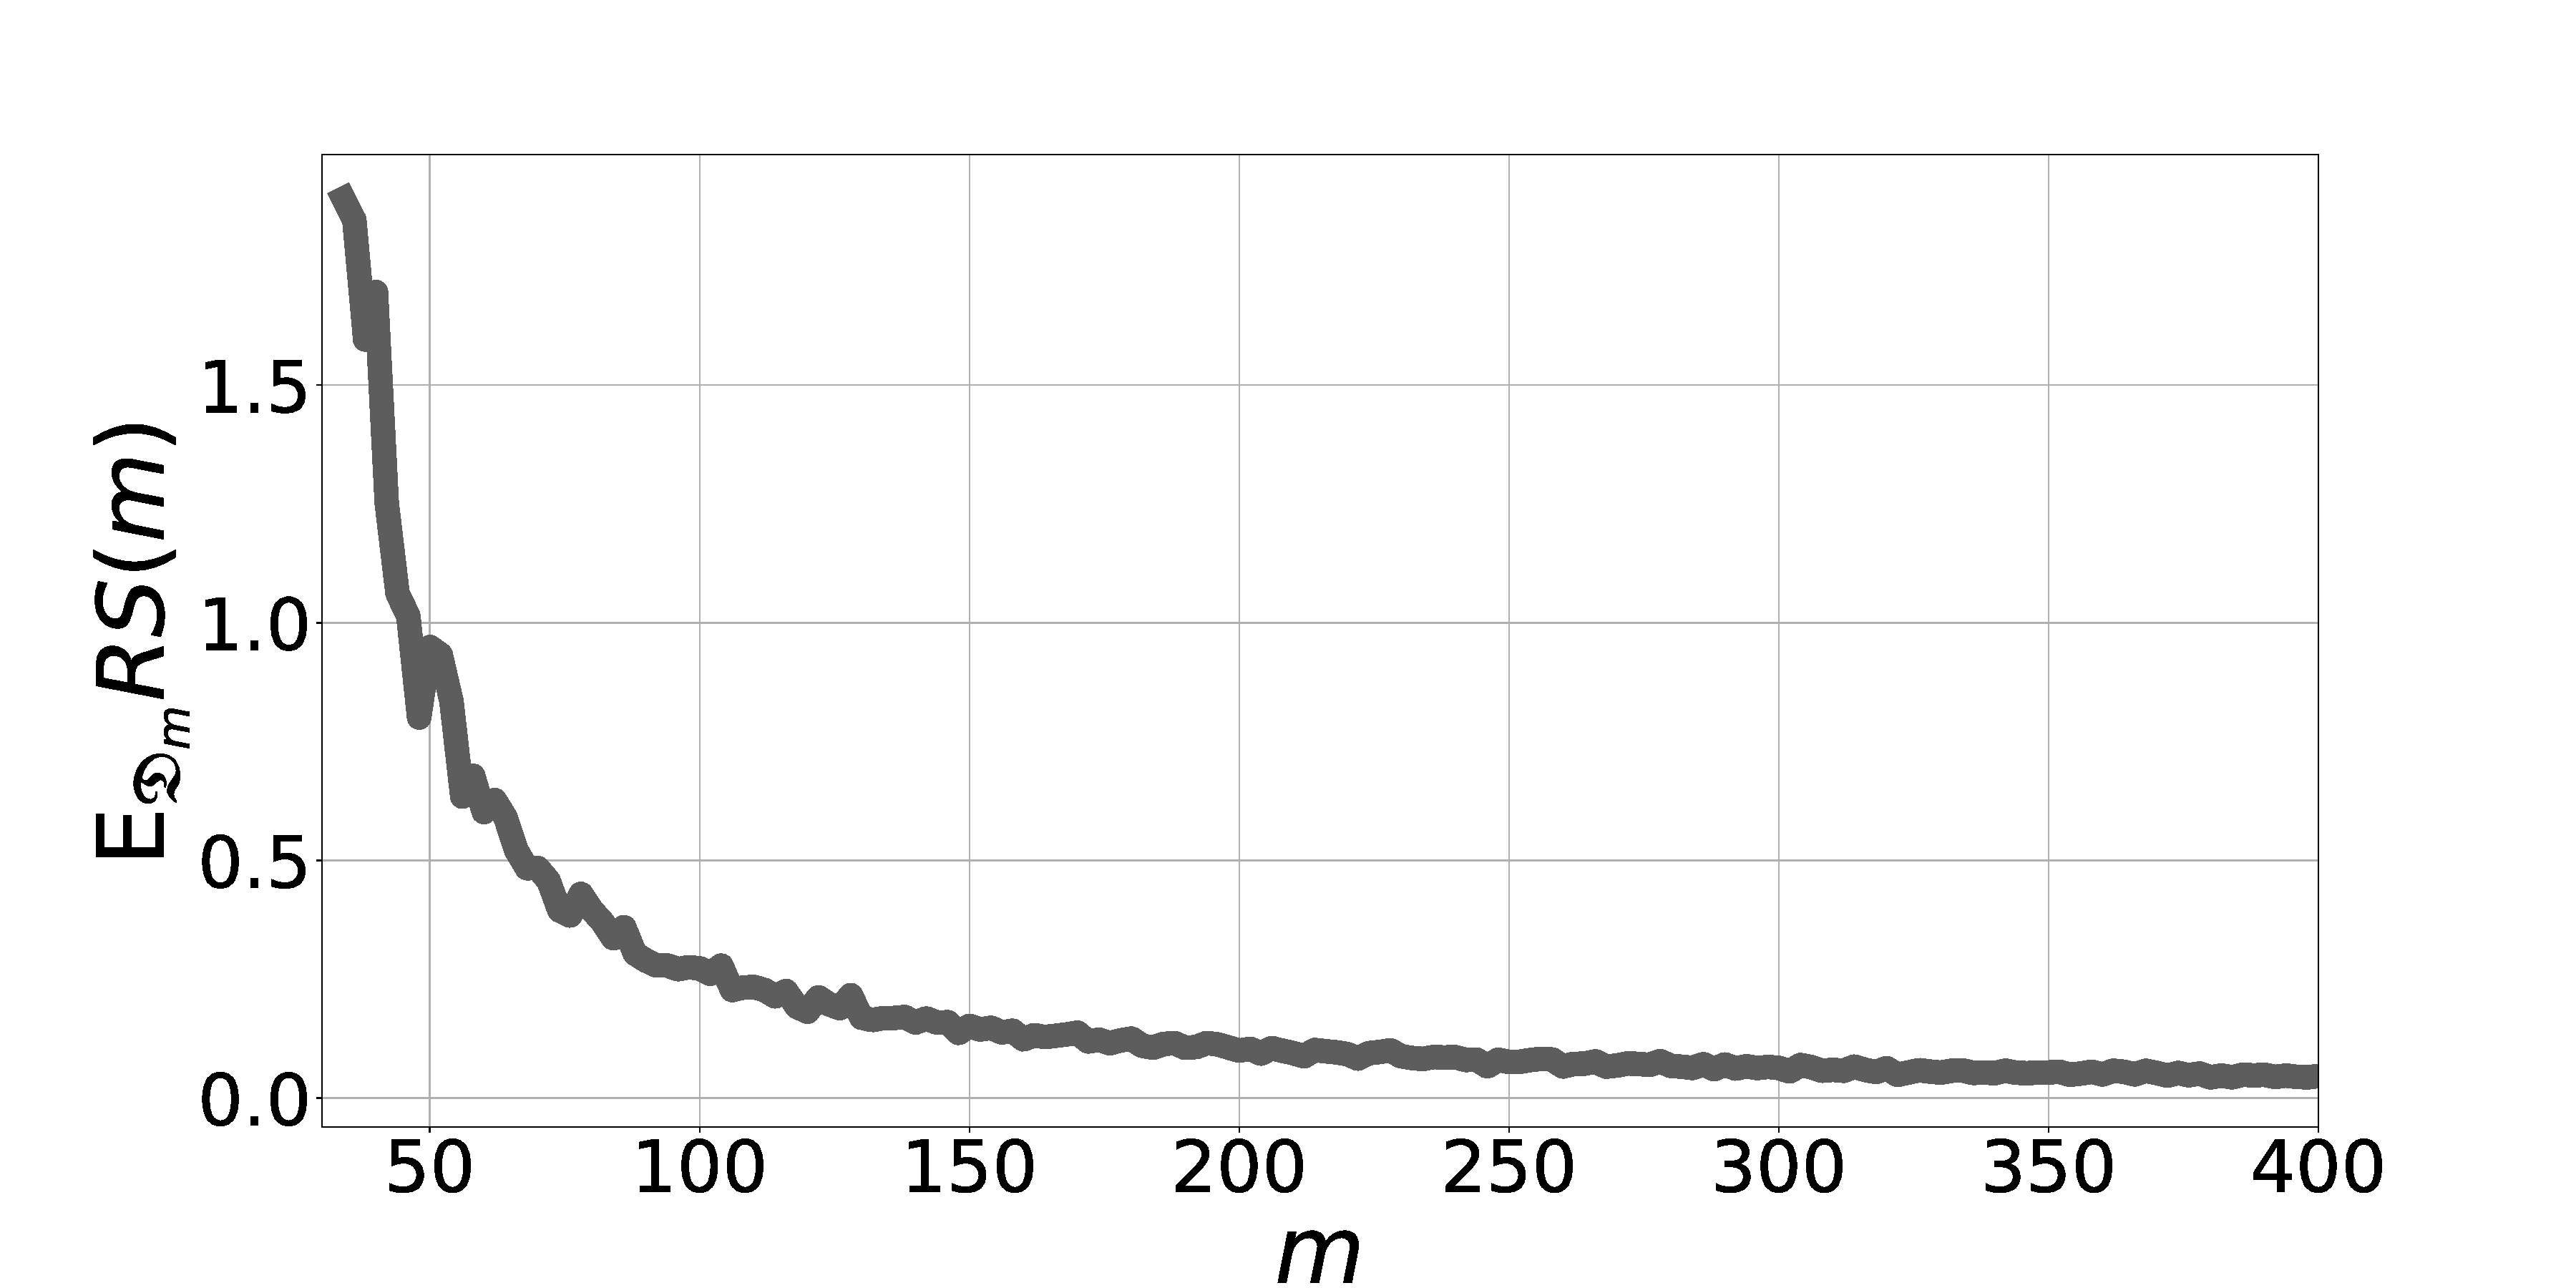
\includegraphics[width=0.49\textwidth]{cross.pdf}}
% \subfloat[APVC ]{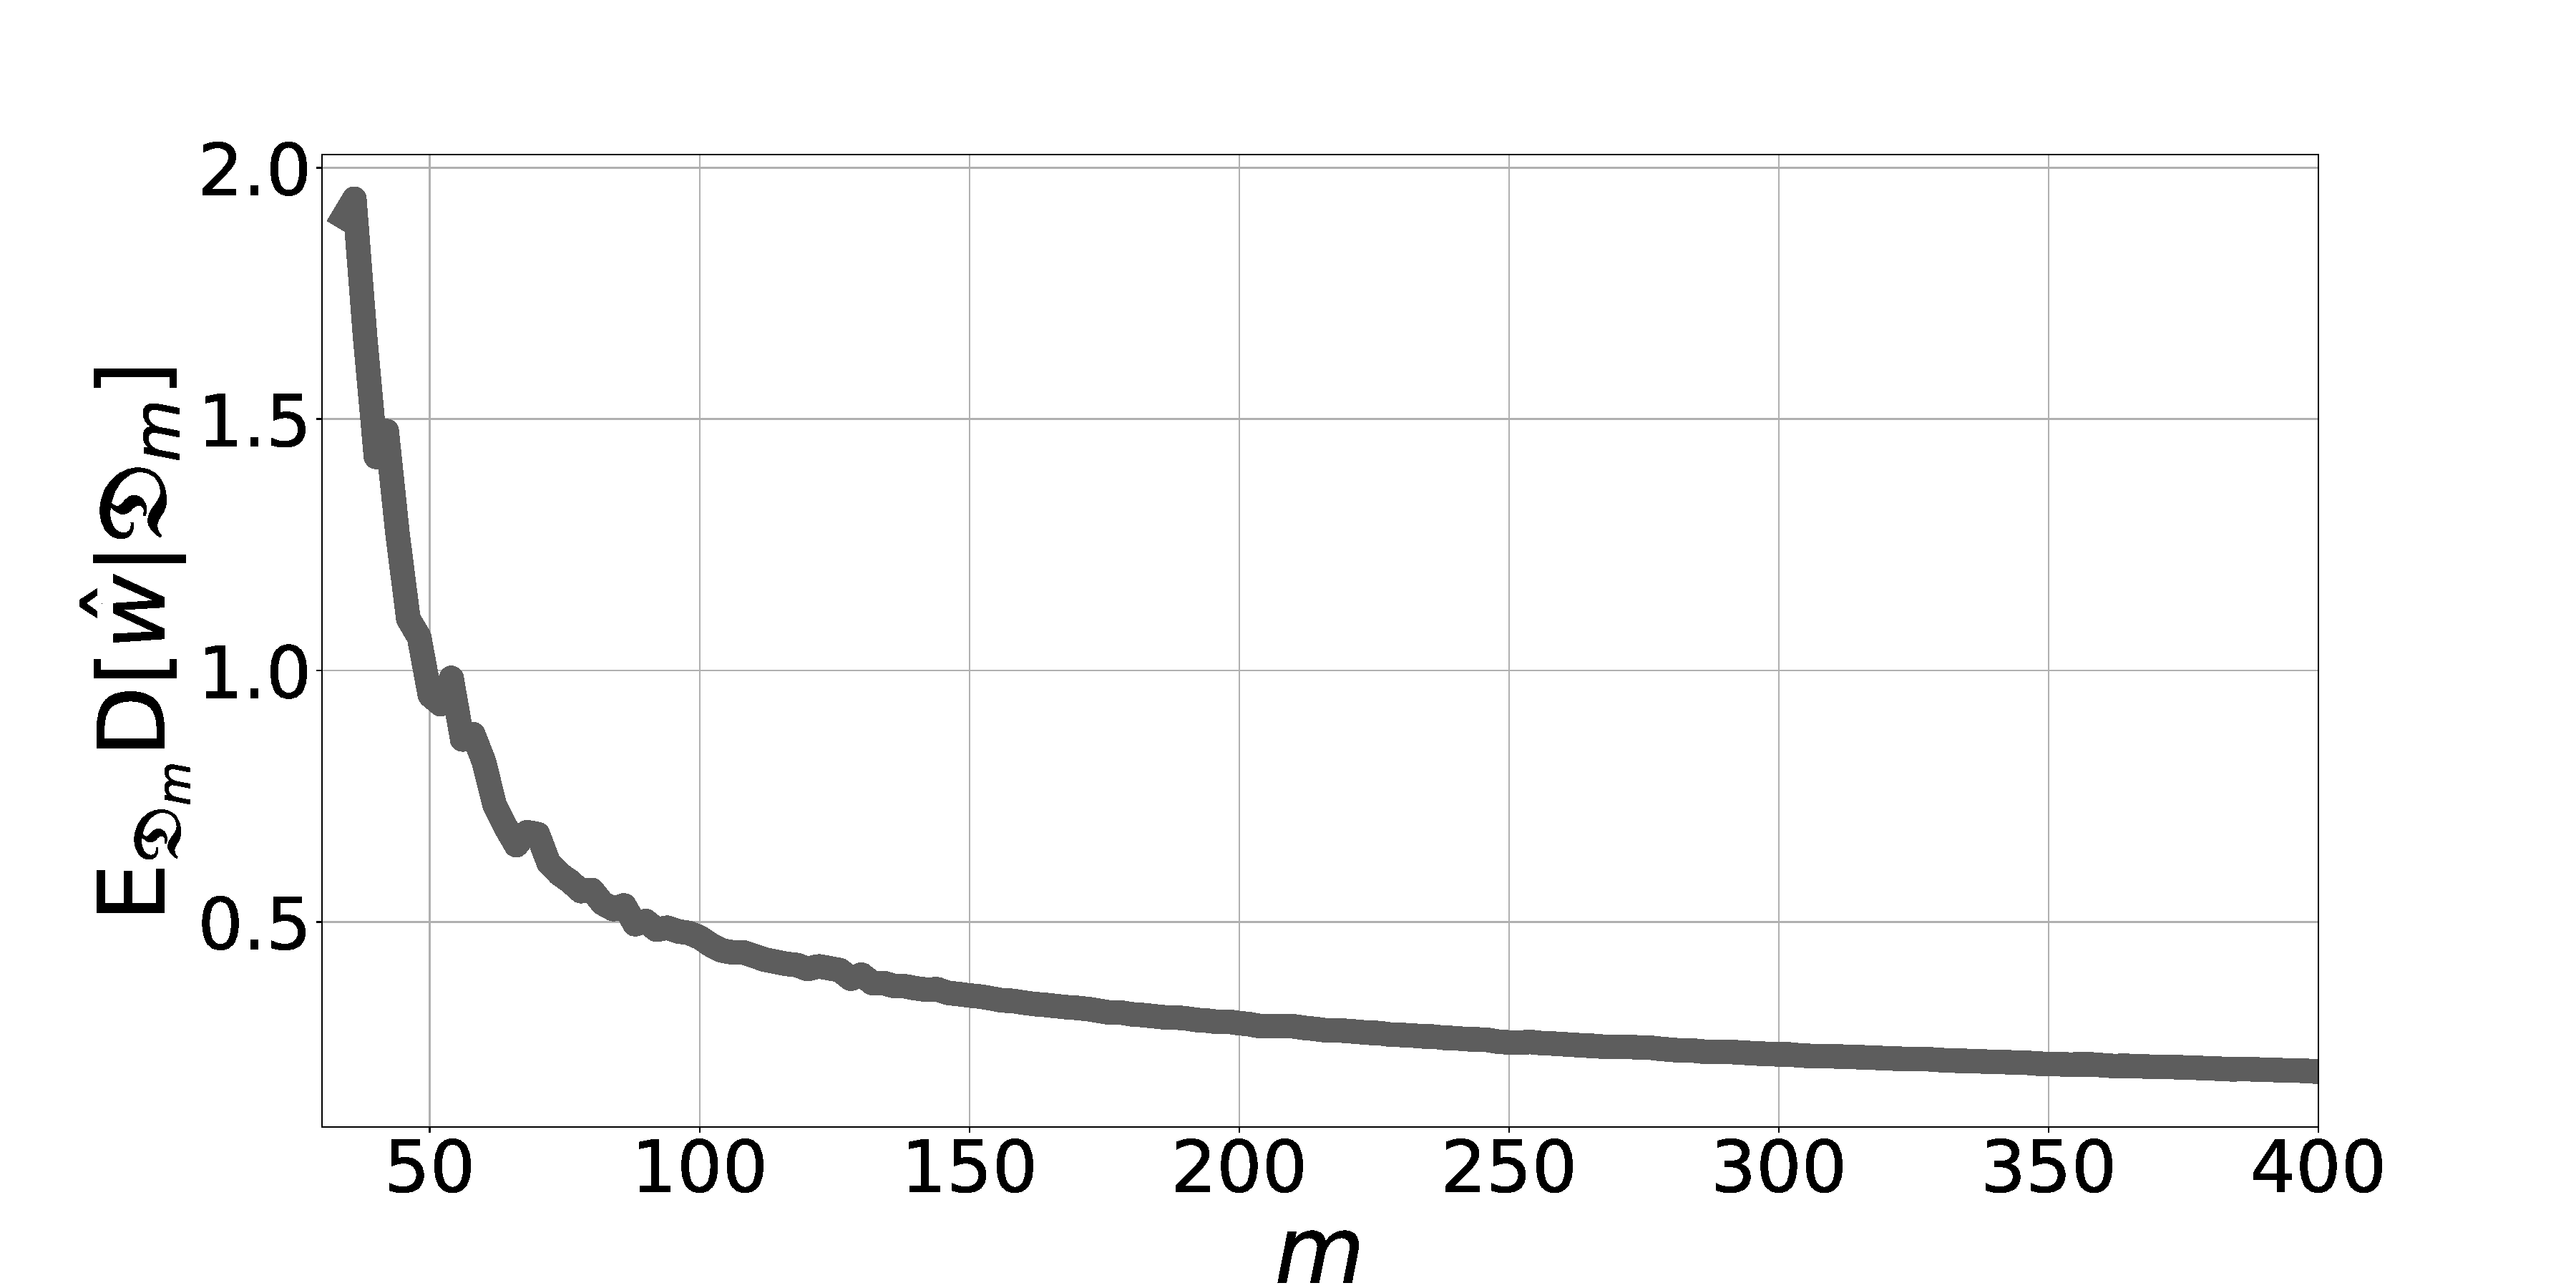
\includegraphics[width=0.49\textwidth]{apvc.pdf}}\\
% \subfloat[ACC ]{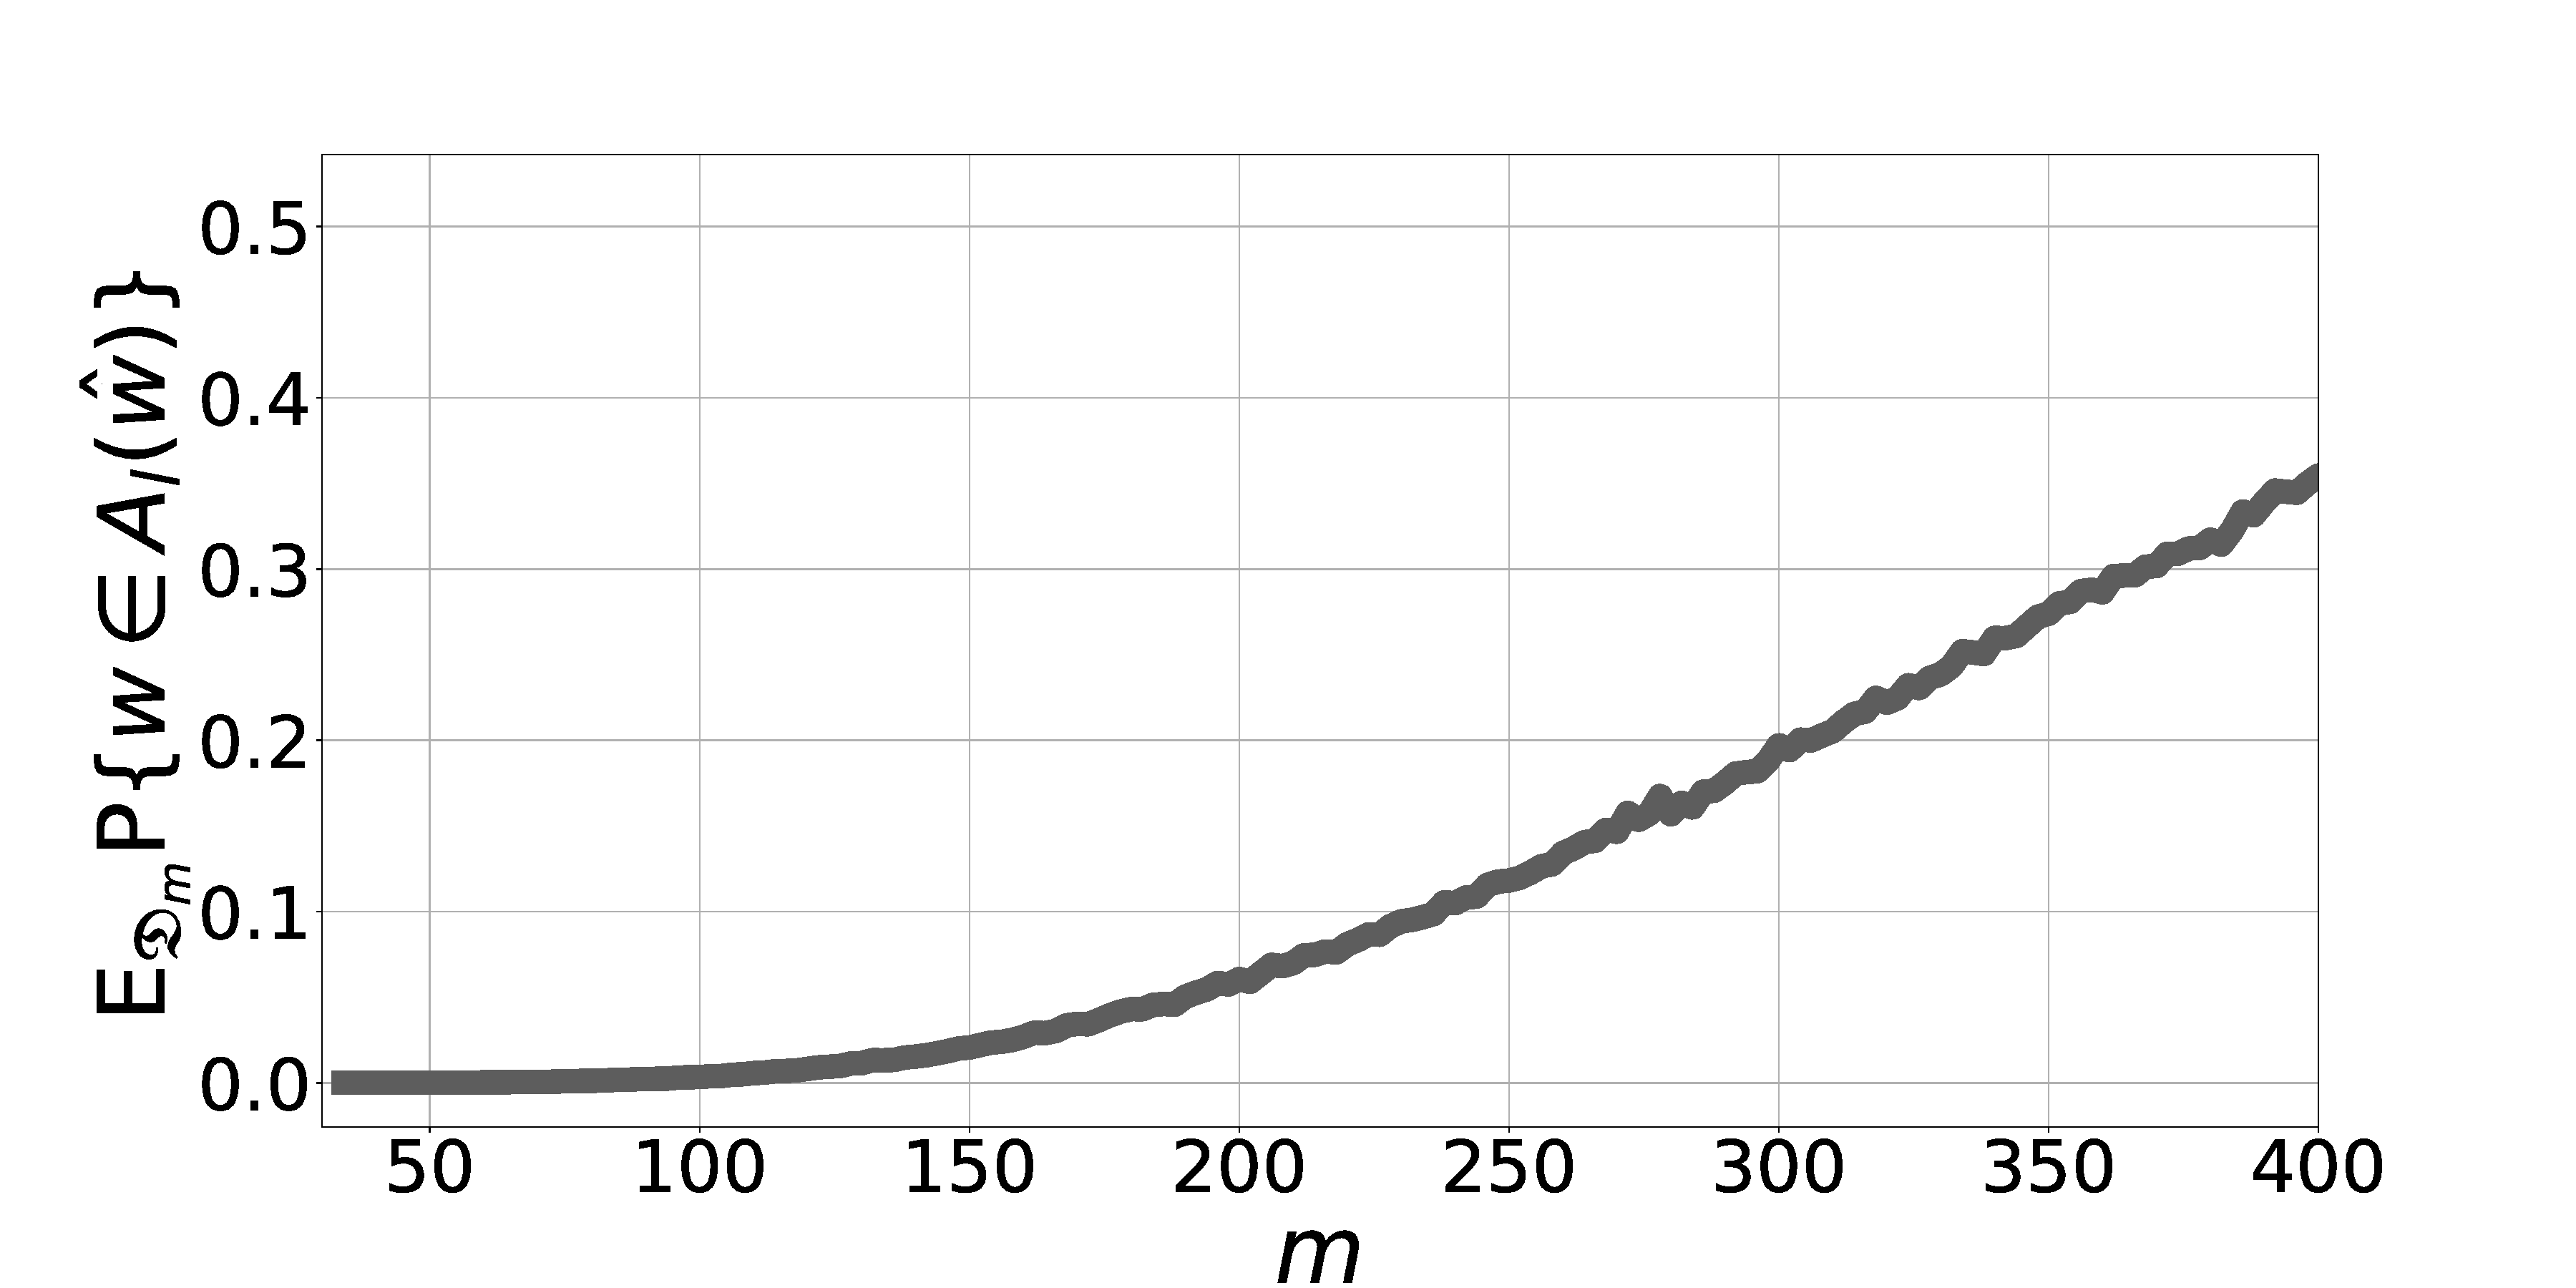
\includegraphics[width=0.49\textwidth]{acc.pdf}}
% \subfloat[ALC ]{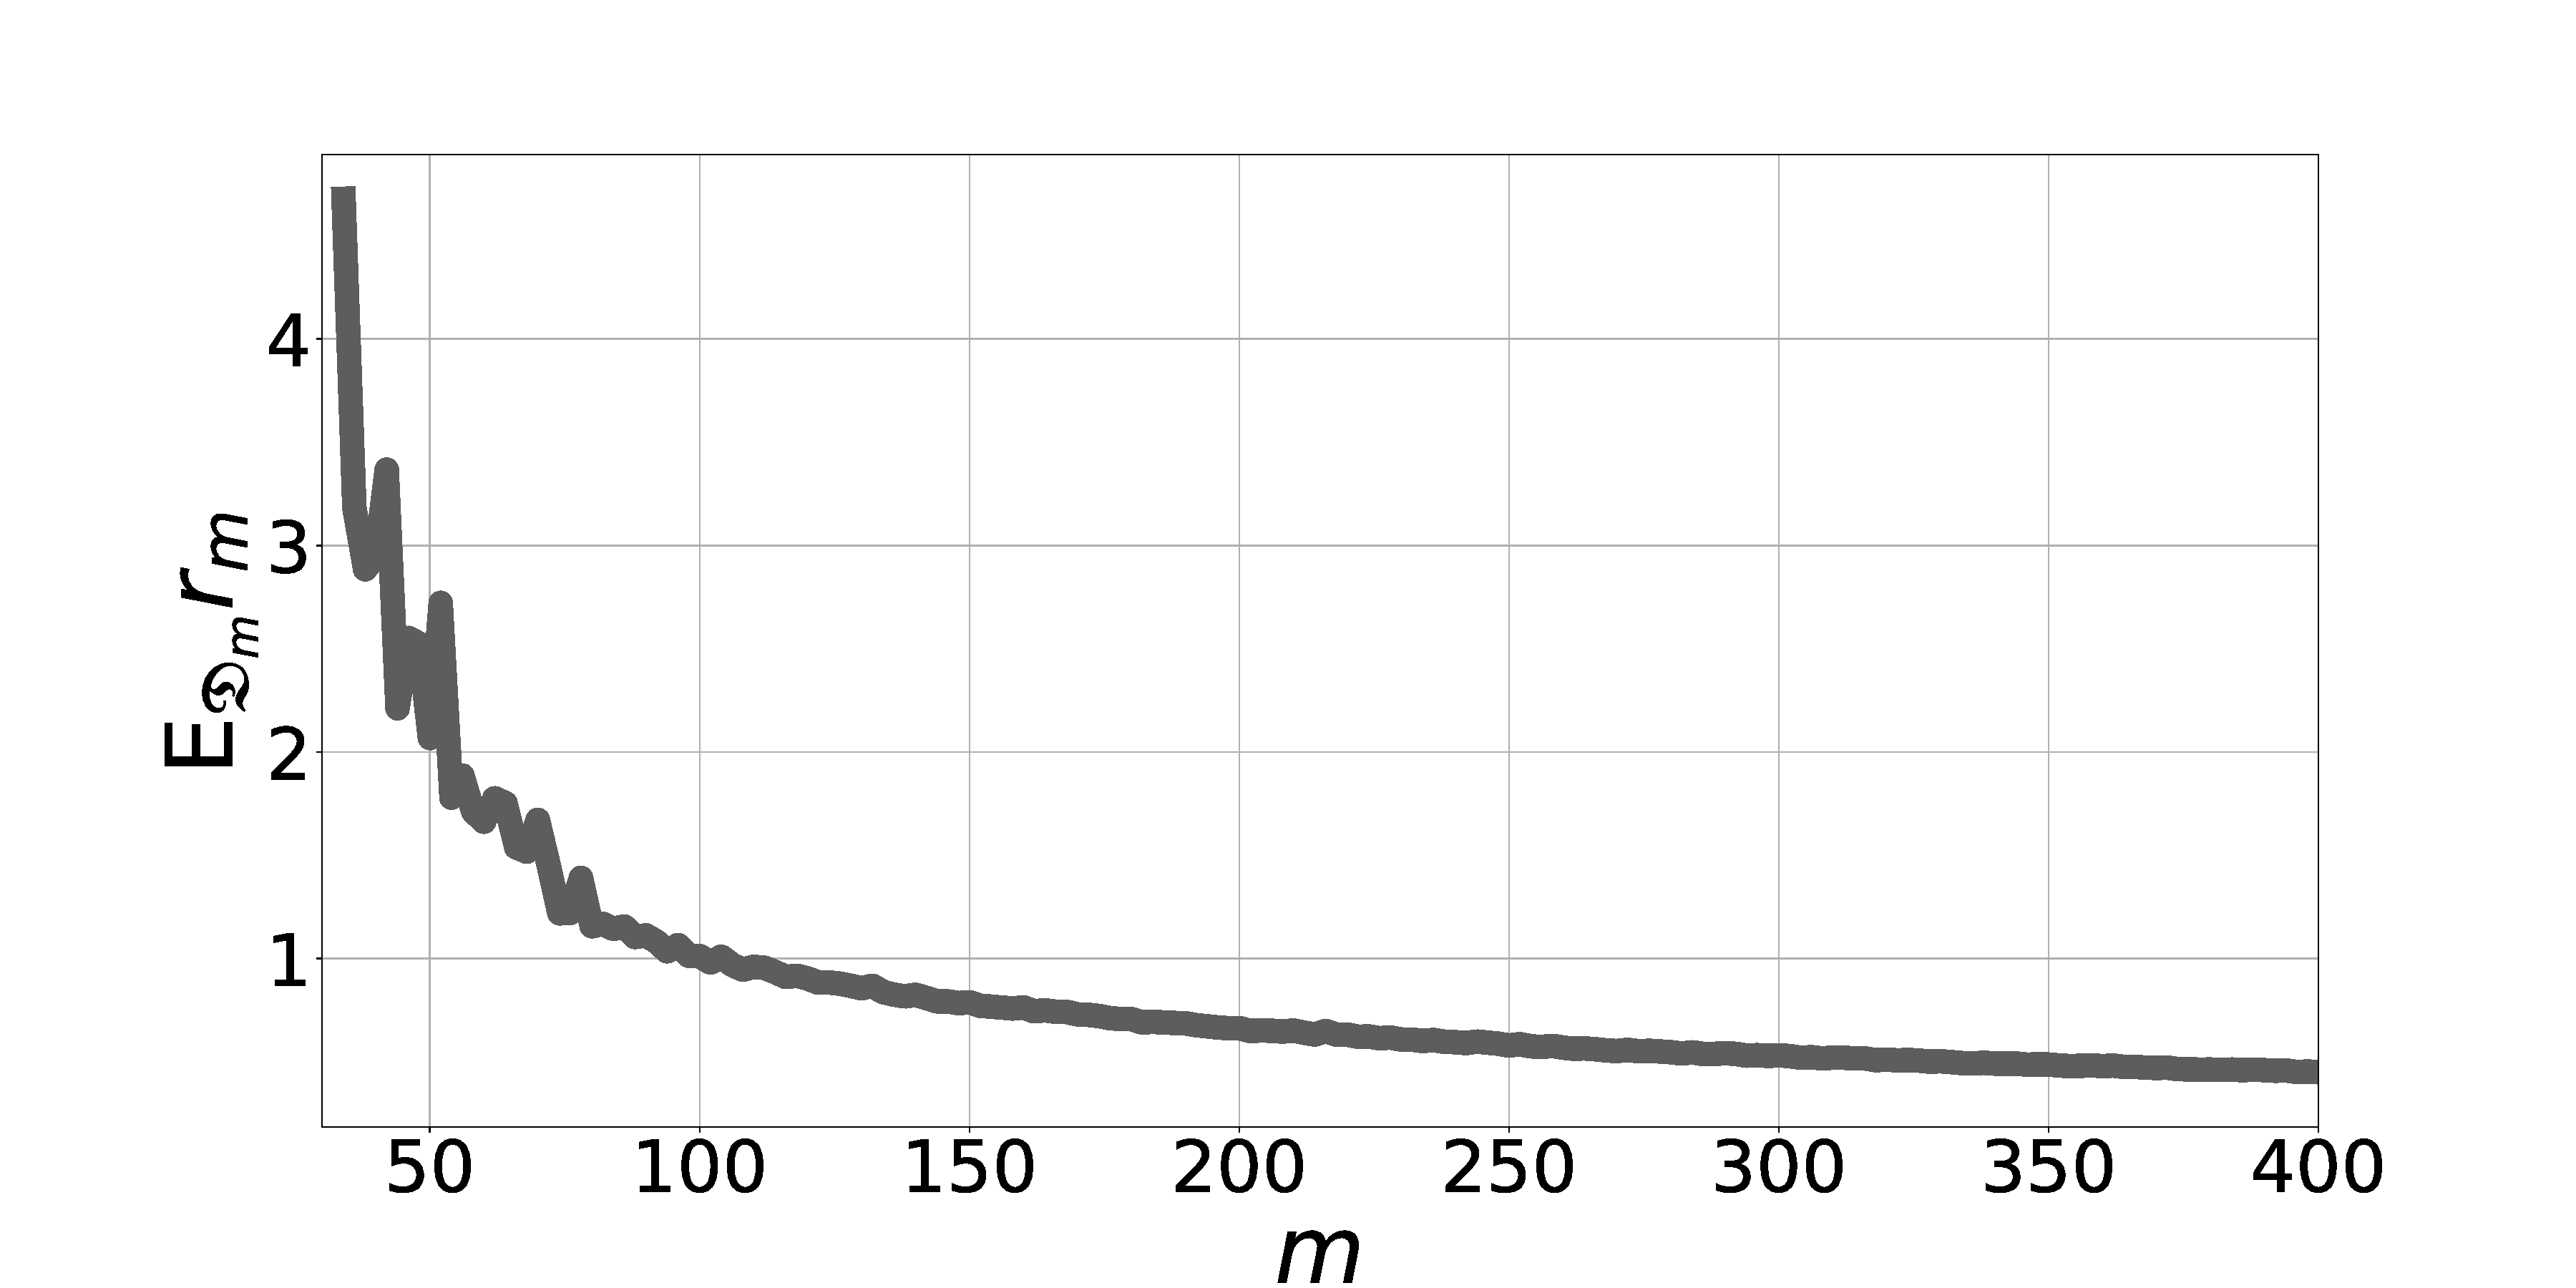
\includegraphics[width=0.49\textwidth]{alc.pdf}}\\
% \subfloat[Bootstrap ]{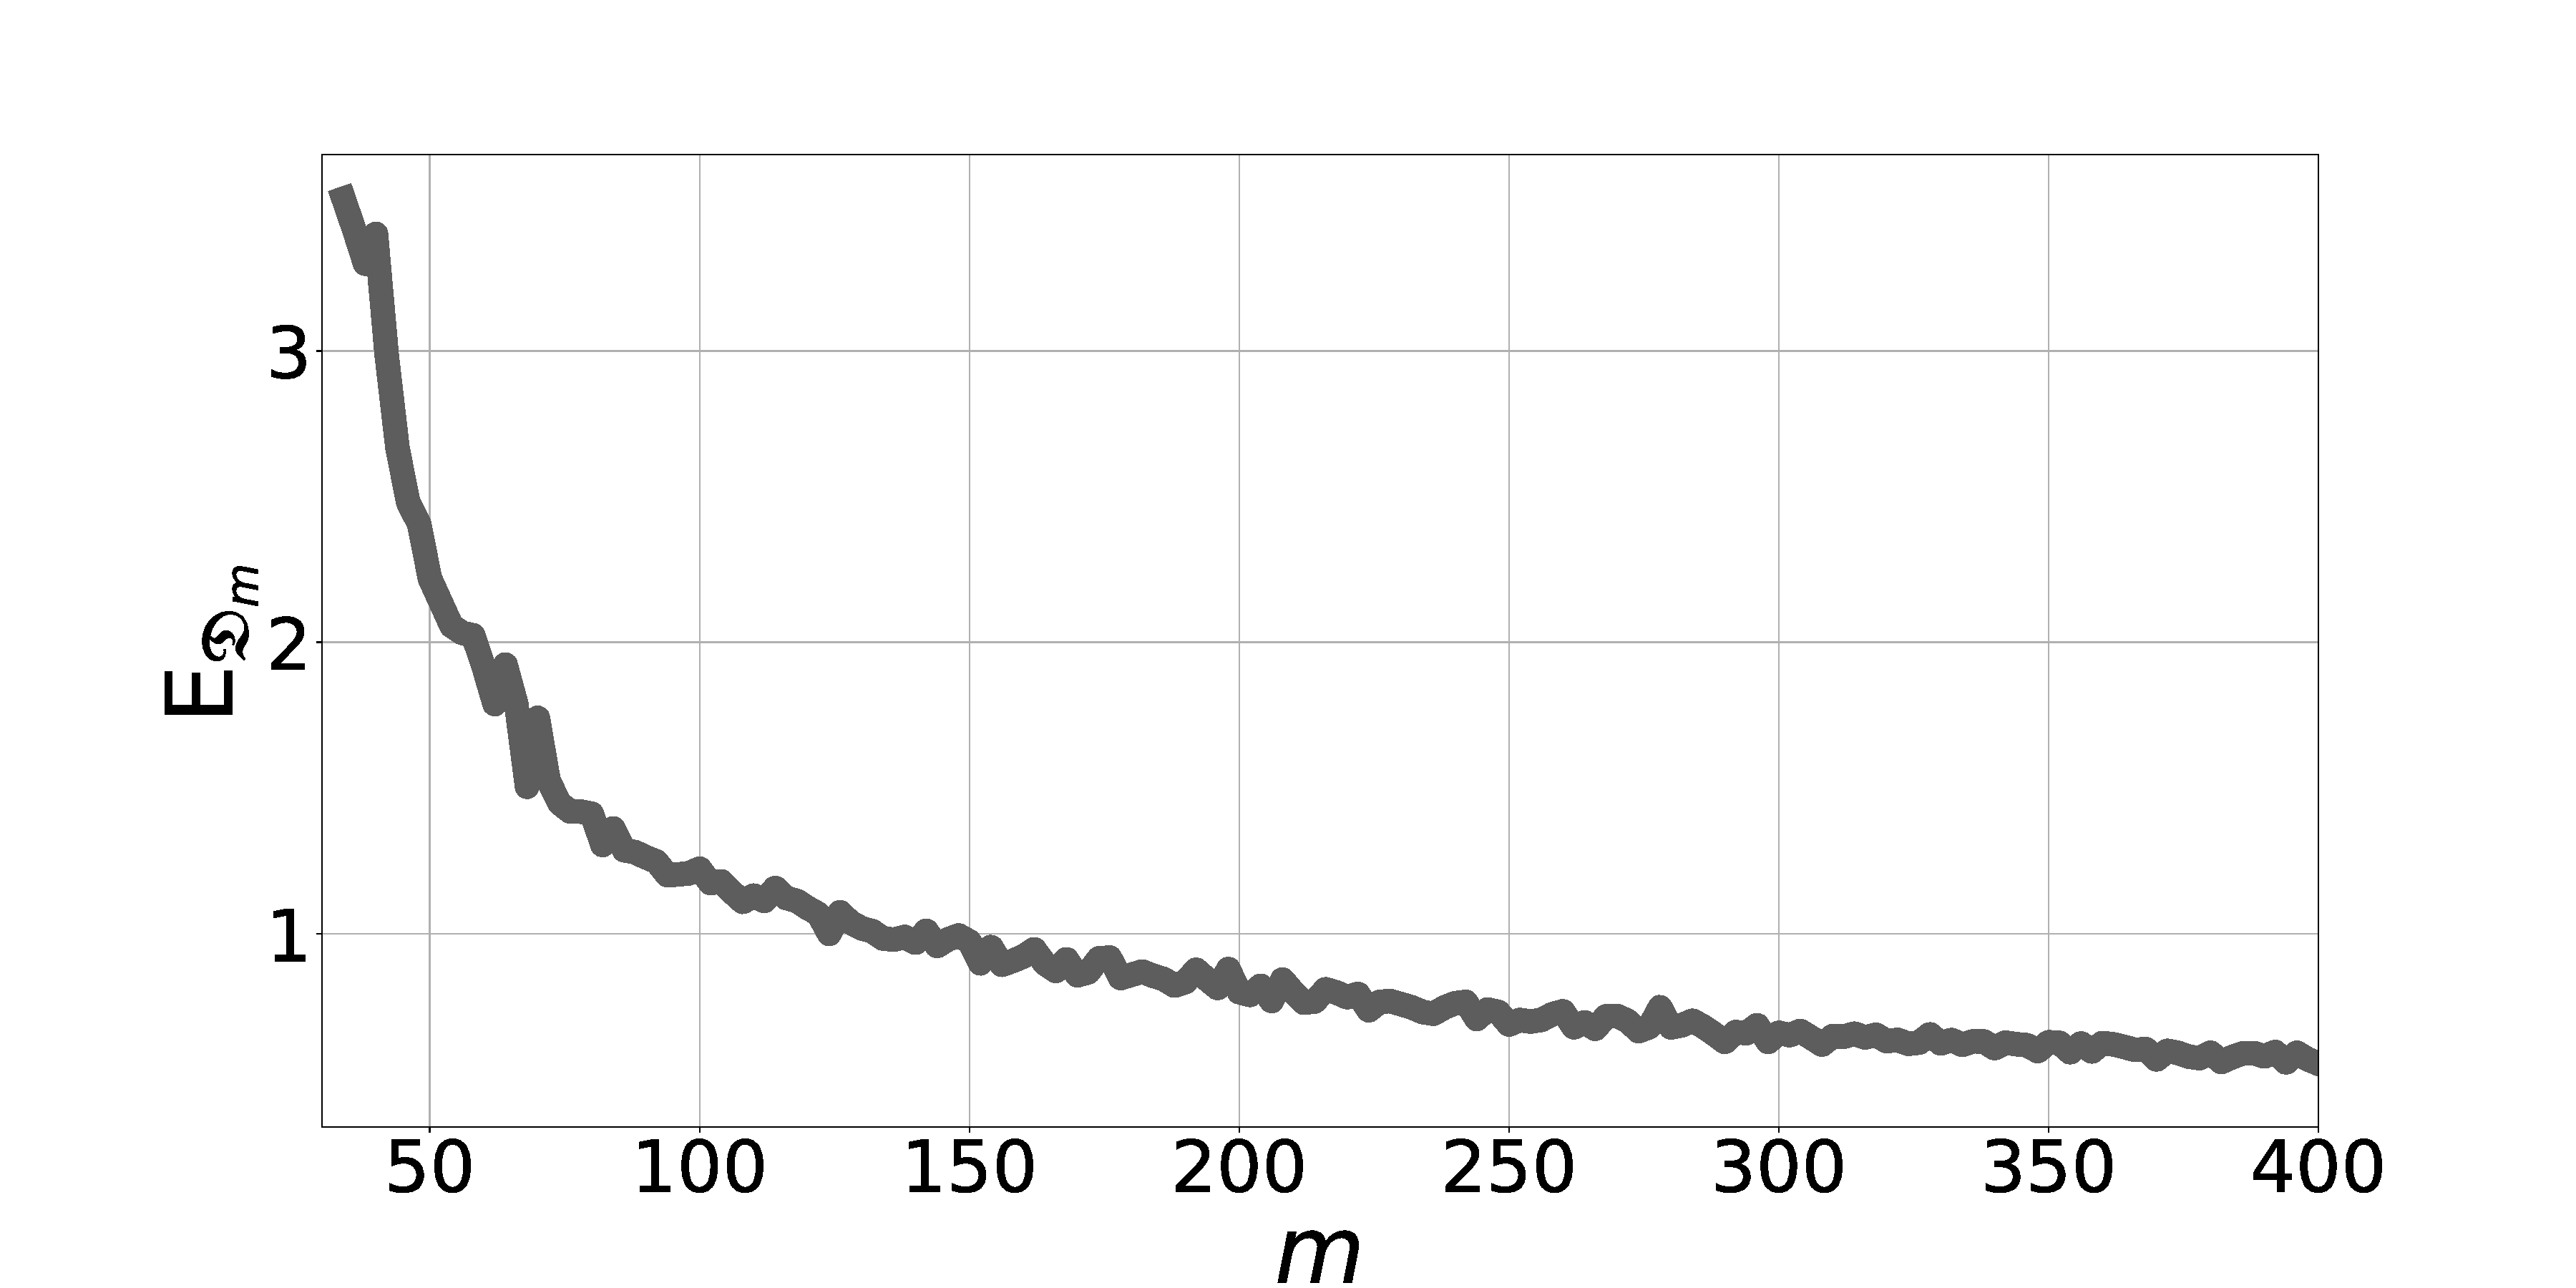
\includegraphics[width=0.49\textwidth]{bootstrap.pdf}}
% \subfloat[KL method ]{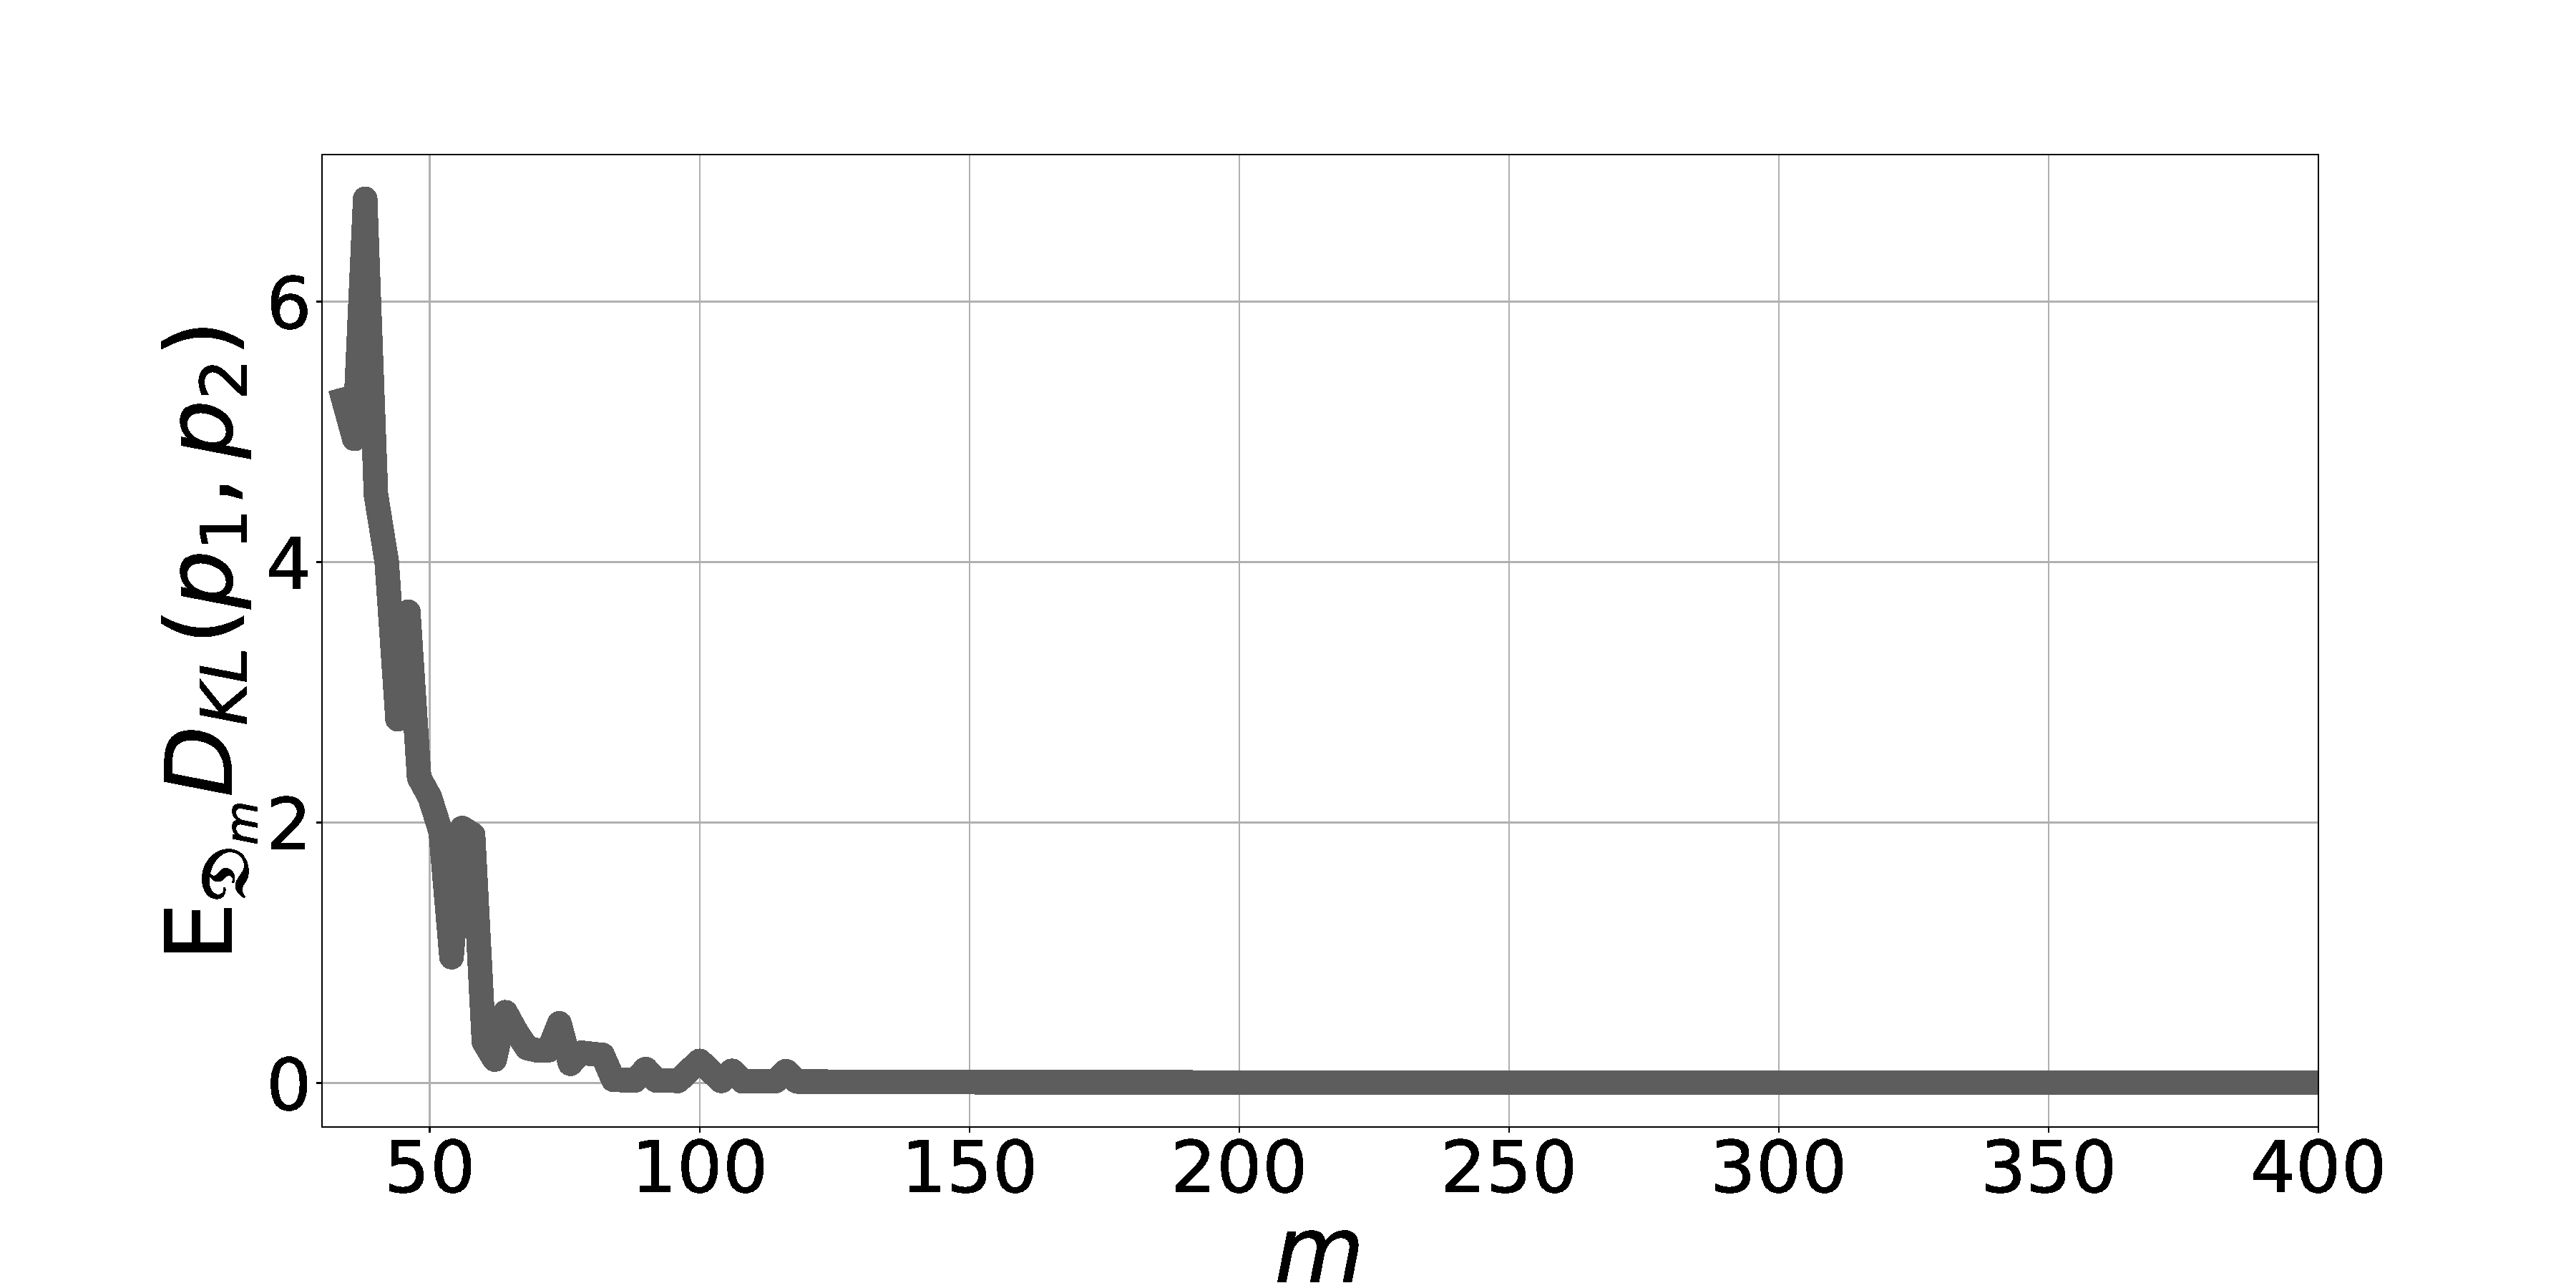
\includegraphics[width=0.49\textwidth]{kl.pdf}}\\
% \subfloat[Utility function ]{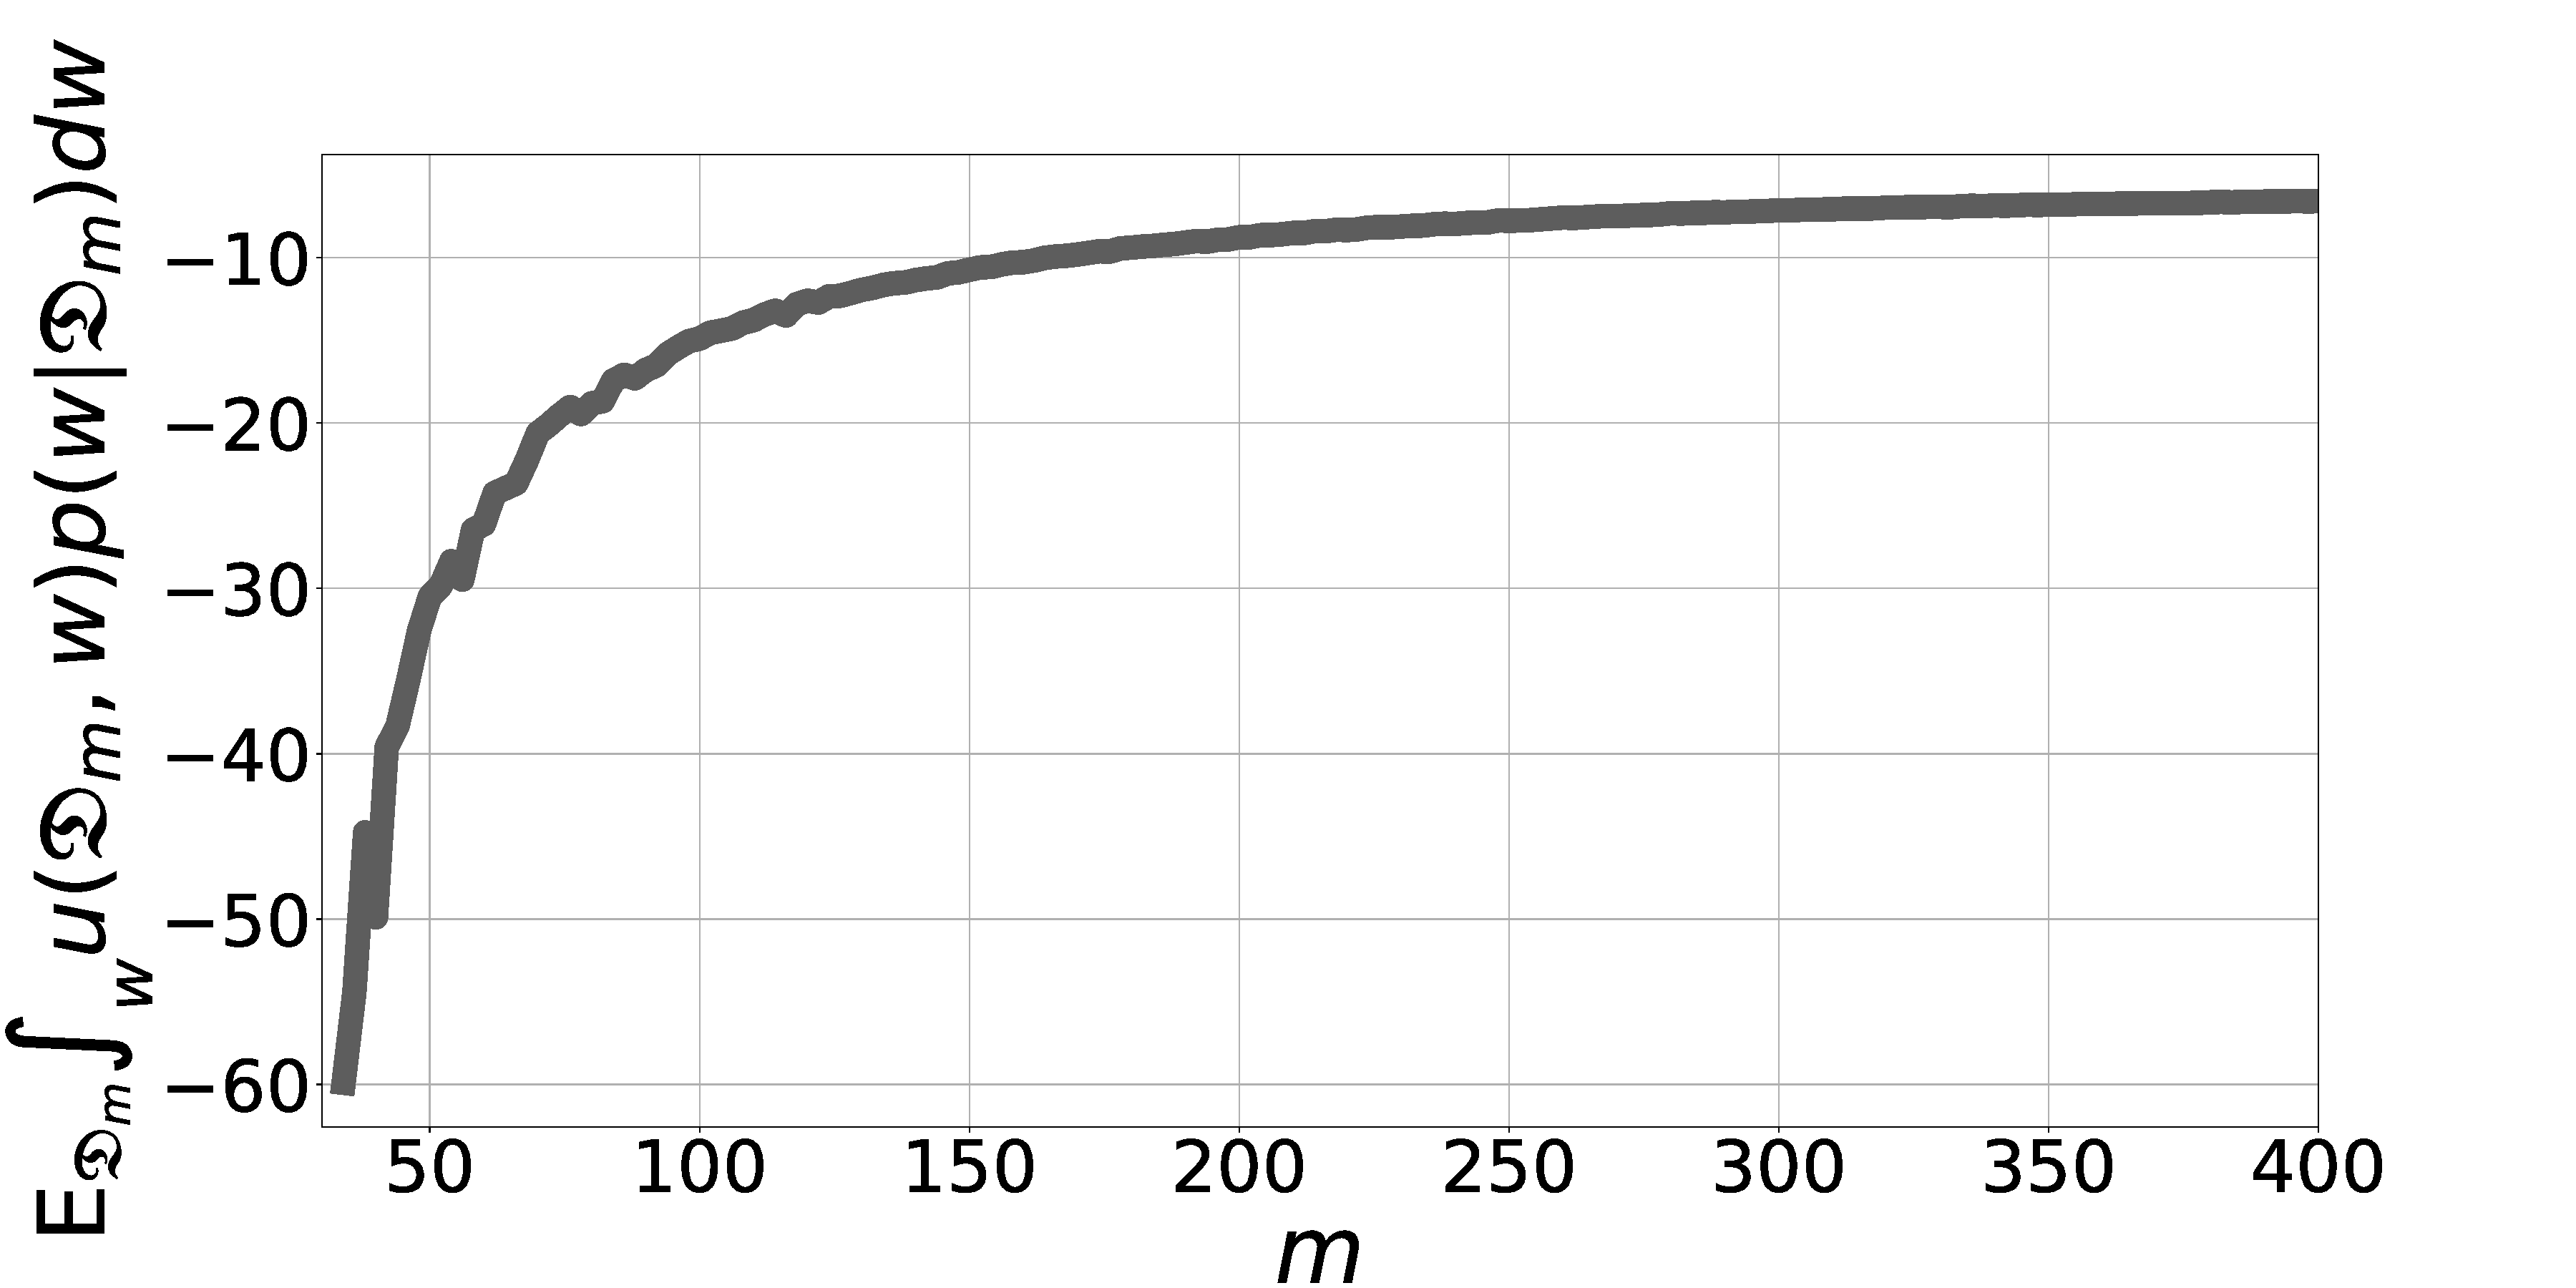
\includegraphics[width=0.49\textwidth]{maxu.pdf}}
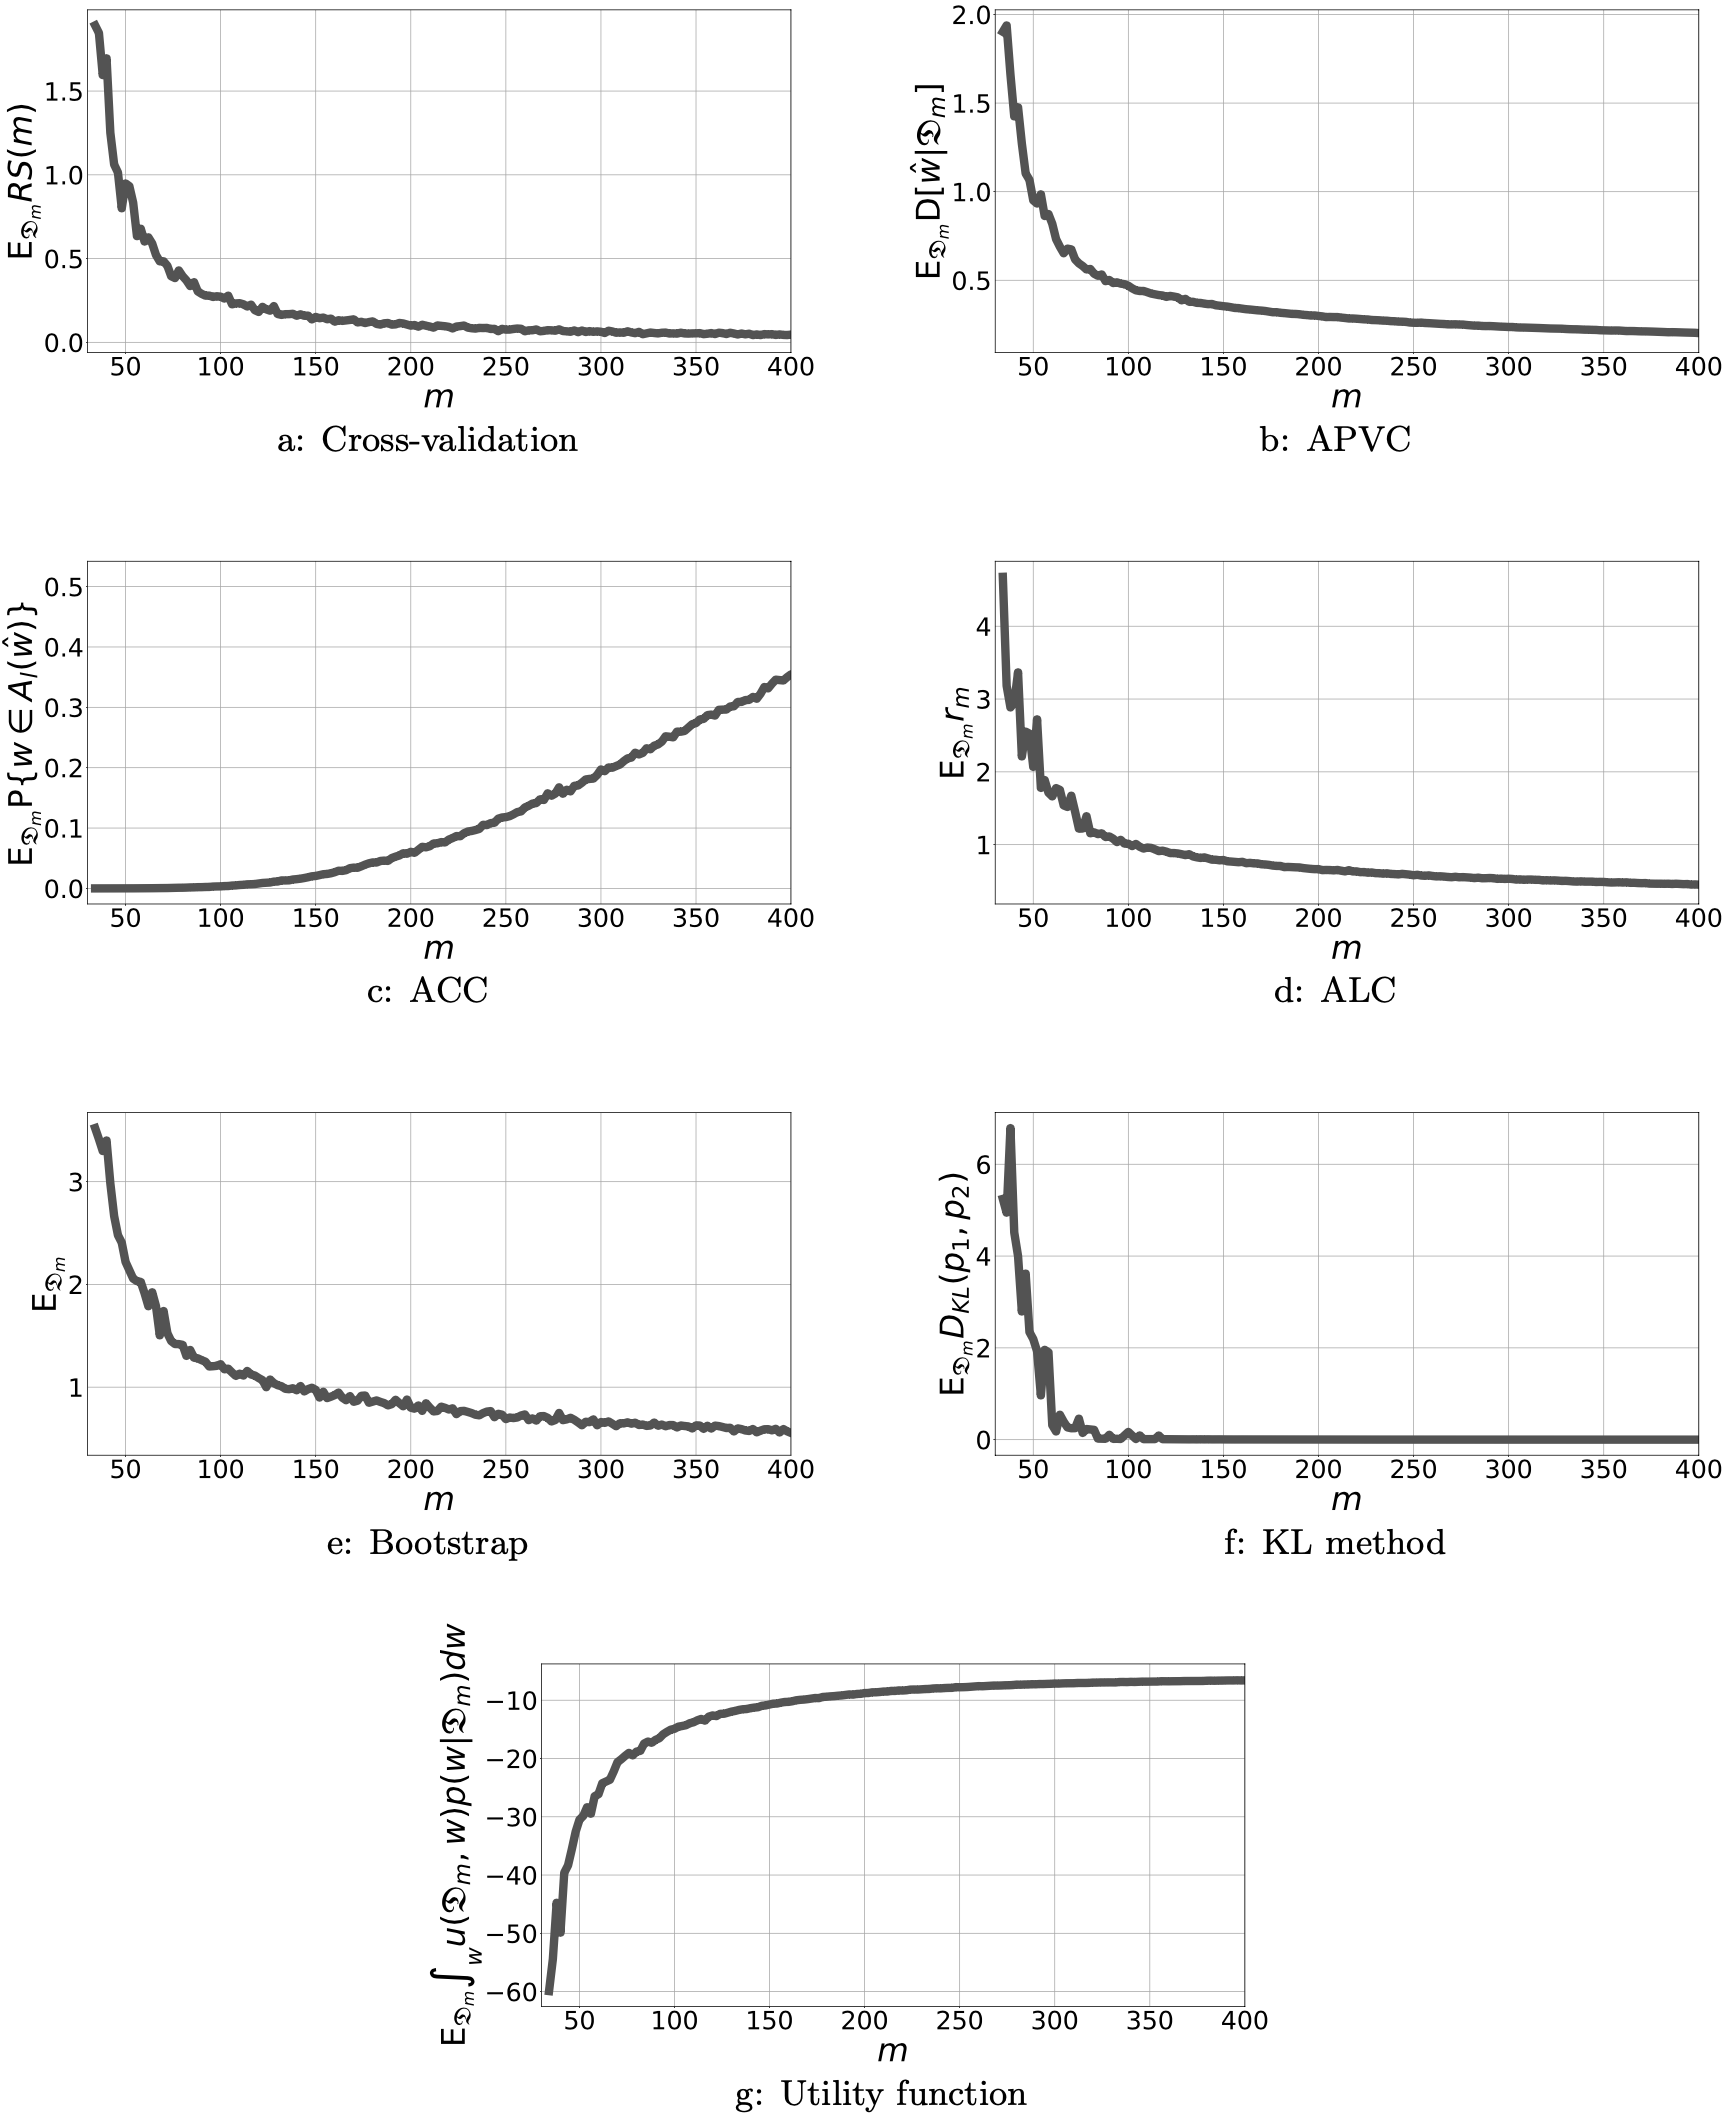
\includegraphics[width=1.0\textwidth]{fig1}
\caption{Dependency of the methods on the available sample size.}
\label{fig1}
\end{figure}

\subsection{Dependency between available sample sets and prediction of their sizes}
This dependency analysis uses the~Boston Housing sample set~\cite{boston}. Given the whole sample set, fix some~$m$ and randomly sample series of bootstrap subsets of size~$m$ from the~initial set. For different values of~$m$ compute values~$m^*$, average them and calculate standard deviation. 
 
\begin{figure}[!htp]
\centering{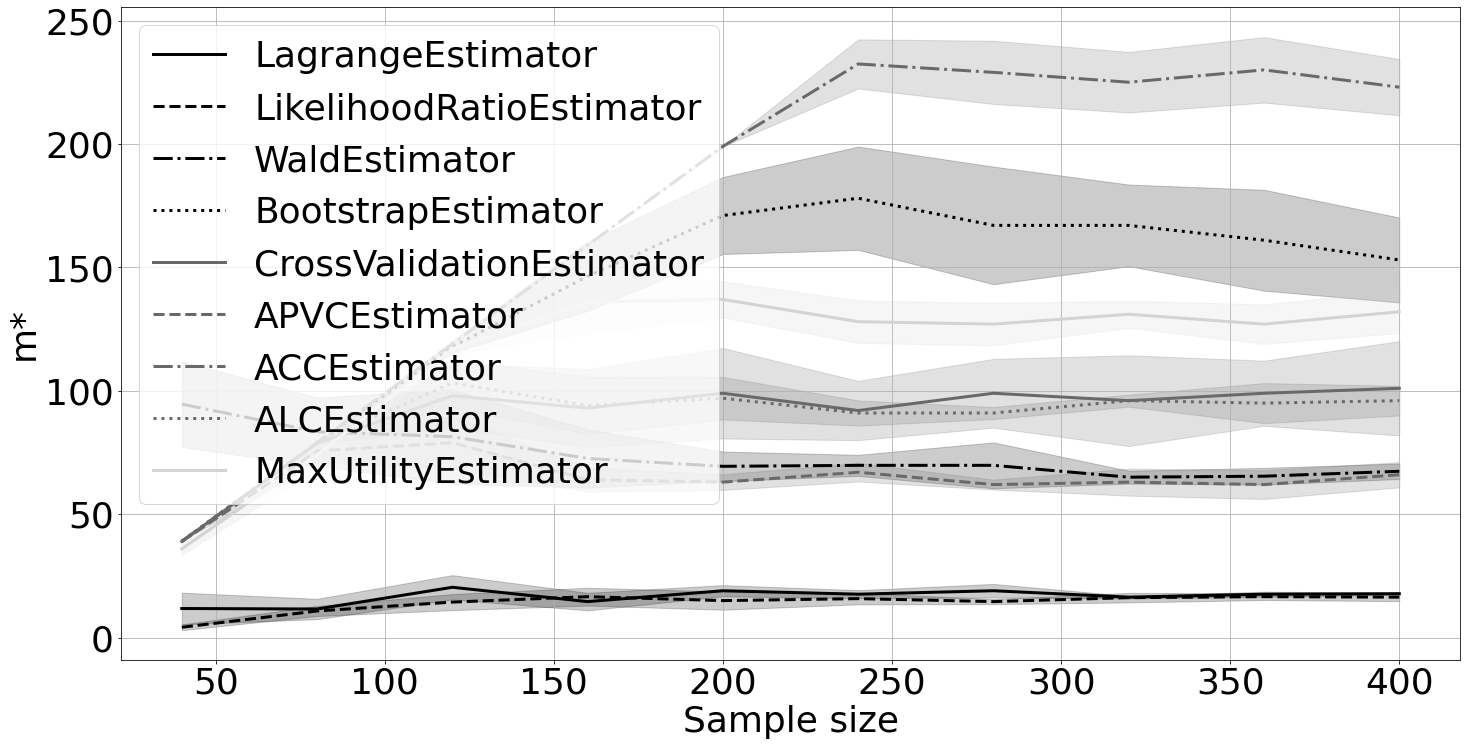
\includegraphics[width=0.85\textwidth]{graphs}}
 \caption{Estimated sample size~$m^*$ versus the available sample size~$m$ for each method.}
\label{fig2}
\end{figure}

Figure~\ref{fig1} shows how the~static value of each method depends on sample size~$m$. %The thresholds for each method are set by the authors.  
Figure~\ref{fig1} demonstrates adequacy of different definitions of sample size sufficiency. Every presented function is monotonous and asymptotically tends to some~constant. Figure~\ref{fig2} shows estimated sample size~$m^*$ for  different sizes~$m$ of the sample set. It shows how methods differ in variance  of estimated values~$m^*$ and how methods behave in case of small size of the sample set. All methods converge and the~result does not depends on the sample size starting from some value of~$m$. 

The small value of the variance of~$m^*$ could be interpreted as stability of the~methods. 
%output with little dependency on a~particular subset of some size. 
Some of the~methods are not able to estimate sufficient sample size unless a sample of  such size is provided. It means that they are useless for prediction of~$m^*$. However, they can be used for retrospective analysis of conducted experiments.

%--- start inclusion
%\subsection{Experiment on subsets}
%The dependence between the~sample size estimation with the~help of a~certain method and the~volume of data available to this method were considered in this exepriment. The constant achieved by the~dependence diagram~$m^*$ on~$m$ is the~forecast of the~optimal sample size method. If this constant is less than~$m$ where the~diagram achieved it, then the~method forecasts the~optimal sample size before obtaining it. Only Lagrange, Wald methods, and the~likelihood ratio method have such property.
%
%\subsection{Experiment on hyperparameter alteration} 
%The alteration of the~sample size estimation depending on the~alteration of certain hyperparameters for Bayesian methods, as well as the~methods based on cross-validation and bootstrap is investigated in this experiment. In order to analyse the~methods behaviour, see the~sample {Boston Housing}, the~other samples have the~identical tendency.
%
%Bayesian methods, as well as the~methods based on cross-validation and bootstrap work on the~basis of a~certain decision rule for a~certain sample function. In~Figure~\ref{fig1}, the~dependence of these functions on the~subset size is shown. As shown in~Figure~\ref{fig1}, these functions are monotonically decreasing, or increasing. The function type of behaviour depends on the~method. By altering the~restrictions set by the~application task, the~sample size which will comply with these restrictions can be altered.
%--- end inclusion

\section{Software}
Methods of sample size estimation listed above are implemented in an easy-to-use Python package. This package is intended for prediction of sufficient sample size at early stages of modelling and for retrospective analysis. This package includes functions for sample size visualization like on Figures~\ref{fig1}~and~\ref{fig2}. The source code is available at \mbox{\url{https://github.com/andriygav/SampleSizeLib}}. The computational experiment code and the sample sets from Table~\ref{table20} is available at \mbox{\url{https://github.com/ttgadaev/SampleSizeEstimation}}.

\section{Conclusion}
This work introduces nine various methods of sufficient sample size estimation. It compares statistic-based, heuristic-based and  Bayesian methods. The~computational experiment compares their numerical properties.

The  experiment shows that  these methods have some restrictions. The statistic-based methods (the~Lagrange test, likelihood ratio, and Wald tests) are asymptotic ones. They cannot be used with a small number of samples. The Bayesian methods, as well as heuristic-based methods (cross-validation and bootstrap) use~ their function on sample set, which requires great number of samples to determine the~sample size. However this kind of methods could be used at the~early stages of data collection.

\section{Future work}
The main problem is to find a~sample size estimation method, that is both interpretable and able to predict~$m^*$ with a~sample set of small insufficient size. One of the prominent solution is to combine one of Bayesian methods  and a statistic-based method, to cope with a sample set of insufficient size.  Our future work is to construct a~statistic, which estimates mean and covariance matrix of the model parameters distribution. This statistic will estimate the sample size of insufficient sample set in terms of one of the~Bayesian definitions of sufficiency. 

\section*{Acknowledgements}
This paper contains results of the project Mathematical methods of intelligent big data analysis, which is carried out within the framework of the Program ``Center of Big Data Storage and Analysis'' of the National Technology Initiative Competence Center. It is supported by the Ministry of Science and Higher Education of the Russian Federation according to the agreement between the M.V. Lomonosov Moscow State University and the Foundation of project support of the National Technology Initiative from 11.12.2018, No 13/1251/2018. This research was supported by RFBR (projects 19-07-01155, 19-07-00885).

\begin{thebibliography}{}
	\bibitem{demidenko2007}
	E. Demidenko, ``Sample size determination for logistic regression revisited,'' Statist. Med. \textbf{26}, 3385--3397 (2007).
	
	\bibitem{self1988}
	S. Self and R. Mauritsen, ``Power/sample size calculations for generalized linear models,'' Biometrics \textbf{44}, 79--86 (1988).
	
	\bibitem{self1992}
	S. Self, R. Mauritsen and J. Ohara, ``Power calculations for likelihood ratio tests in generalized linear models,'' Biometrics \textbf{48}, 31--39 (1992).
	
	\bibitem{shieh2000}
	G. Shieh, ``On power and sample size calculations for likelihood ratio tests in generalized linear models,'' Biometrics \textbf{56}, 1192--1196 (2000).
	
	\bibitem{kloek1975}
	T. Kloek, ``Note on a~large-sample result in specification analysis,'' Econometrica \textbf{43}, 933--936 (1975).
	
	\bibitem{shieh2005}
	G. Shieh, ``On power and sample size calculations for Wald tests in generalized linear models,'' Journal of Statistical Planning and Inference \textbf{128}, 43--59 (2005).

	\bibitem{motrenko2014}
	A. Motrenko, V. Strijov and G. Weber, ``Sample size determination for logis
	
	ression,'' Journal of Computational and Applied Mathematics \textbf{255}, 743--752 (2014).
	
	\bibitem{qumsiyeh2013}
	M. Qumsiyeh, ``Using the~bootstrap for estimation the~sample size in statistical experiments,'' Journal of modern applied statistical methods \textbf{8}, 305--321 (2013).
	
	\bibitem{lindley1997}
	D. Lindley, ``The choice of sample size,'' Statistician \textbf{46}, 129--138 (1997).
	
	\bibitem{rubin1998}
	D. Rubin and H. Stern, ``Sample size determination using posterior predictive distributions,'' Sankhya: The Indian Journal of Statistics Special Issue on Bayesian Analysis \textbf{60}, 161--175 (1998).

	\bibitem{wang2002}
	F. Wang and A. Gelfand, ``A Simulation-based Approach to Bayesian Sample Size Determination for Performance under a~Given Model and for Separating Models,'' Statistical Science \textbf{17}, 193--208 (2002).
	
	\bibitem{joseph1997}
	L. Joseph, R. Berger and P. Be'lisle, ``Bayesian and mixed bayesian likelihood criteria for sample size determination,'' Statistician \textbf{16}, 769--781 (1995).
	
	\bibitem{joseph1995}
	L. Joseph, D. Wolfson and R. Berger, ``Sample size calculations for binomial proportions via highest posterior density intervals,'' Statistical Medicine \textbf{44}, 143--154 (1997).
	
	\bibitem{servo}
	J. Quinlan, ``Learning with continuous classes,'' in \emph{Proc. 5th Australian Joint Conference on AI} (1992), pp.~343--348.
	
	\bibitem{boston}
	D. Harrison and D. Rubinfeld, ``Hedonic prices and the~demand for clean air,'' Economics and Management \textbf{5}, 81--102 (1978).

\end{thebibliography}
\end{document}